\title{Seismic noise attenuation using an online subspace tracking algorithm}
\author{Yatong Zhou\footnotemark[1] and Shuhua Li\footnotemark[1] and Dong Zhang\footnotemark[2] and Yangkang Chen\footnotemark[3]}

\address{
\footnotemark[1] School of Electronic and Information Engineering \\
Hebei University of Technology \\
Xiping Road No. 5340, Beichen District\\
Tianjin, China, 300401 \\
zyt\_htu@126.com \\ 
\footnotemark[2] Departments of Imaging Physics \\
Delft university of technology \\
D.Zhang-3@tudelft.nl \\
%331334826@qq.com
%liutingjiy@126.com \\
%+86-18810415565 
%\footnotemark[2] Department of Physics\\
%University of Alberta\\
%Edmonton, AB T6G 2R3, Canada \\
%xjyshl@sina.com \\
\footnotemark[3] Previously: Bureau of Economic Geology \\
John A. and Katherine G. Jackson School of Geosciences \\
The University of Texas at Austin \\
University Station, Box X \\
Austin, TX 78713-8924 \\
Currently: National Center for Computational Sciences \\
Oak Ridge National Laboratory \\
One Bethel Valley Road, \\
Oak Ridge, TN 37831-6008 \\
Email: chenyk2016@gmail.com\\
%University Station, Box X\\
%Austin, TX 78713-8924, USA \\
%Email: ykchen@utexas.edu
}
\DeclareRobustCommand{\dlo}[1]{\ifthenelse{\boolean{@revd}}{}{}}
\DeclareRobustCommand{\wen}[1]{%
  \ifthenelse{\boolean{@revd}}{\textcolor{black}{#1}}{#1}}
  
\lefthead{Zhou et al.}
\righthead{Online subspace tracking algorithm}
	
\begin{abstract}
We propose a new low-rank based noise attenuation method using an efficient  algorithm for tracking subspaces from highly corrupted seismic observations. The subspace tracking algorithm requires only basic linear algebraic manipulations. %Each subspace update can be performed in linear time in the dimension of the subspace. 
The algorithm is derived by analyzing incremental gradient descent on the Grassmannian manifold of subspaces. When the multi-dimensional seismic data is mapped to a low-rank space, the subspace tracking algorithm can be directly applied to the input low-rank matrix to estimate the useful signals. Since the subspace tracking algorithm is an online algorithm, it is more robust to random noise than traditional \wen{truncated} singular value decomposition (TSVD) based subspace tracking algorithm. Compared with the state-of-the-art algorithms, the proposed denoising method can obtain better performance. More specifically, the proposed method outperforms the \wen{TSVD-based} singular spectrum analysis (SSA) method in causing less residual noise and also in saving half of the computational cost. Several synthetic and field data examples with different levels of complexities demonstrate the effectiveness and robustness of the presented algorithm in rejecting different types of noise including random noise, spiky noise, blending noise, and coherent noise. 
\end{abstract}

\maketitle



\section{Introduction}
Seismic data is inevitably corrupted by different types of noise. The existence of noise in the prestack seismic data masks useful signals, affects the amplitude information, and thus causes unreliable inversion results. Even in post-stack seismic data, the existence of noise will affect interpretation result which directly links the seismic images with subsurface oil \& gas reservoirs \cite[]{yanfei2011,yangkangthesis,pstmjse2016,jsewe2016,yangkang2016emd,shuwei2016vscan}. A successful separation between useful reflection signals and unwanted noise is a long standing problem in the area of seismic data processing and greatly affects the fidelity of subsequent seismic imaging and geophysical inversion, like amplitude-variation-with-offset (AVO) inversion, full waveform inversion, attenuation estimation, and geological interpretation \cite[]{jsehessian2015,jserugekutta2016,jsepssp2016,jsedecon2016,fangyu2016,qianping2016,mostafa2016geo,mostafa2016jag,mostafa2016bssa,zhaoyu2016,qushan2016seg,jingnan2017,qushan2017,saleh2017,mostafa2017geo}. Effectively rejecting the cross-talke interference caused in the simultaneous-source seismic acquisition also plays a significant role in tremendously saving the data recording cost \cite[]{berkhout2008,qushan2014,abma2015,qushan2015,shaohuan2015,yangkang2015pnmo,yangkang2015image,yangkang2015dbortho,qushan2016,yangkang2017lsrtm,shaohuan2017,shaohuan2017jag,shaohuan2017gji,yatong2017}.

Over the past few decades, a large number of denoising methods for random noise have been developed and widely applied in practice. The simplest denoising method is by stacking the seismic data along the offset direction \cite[]{Mayne62,guochang2009,wencheng2015stack}. By stacking the useful signals from multiple traces and multiple directions (e.g., offset and midpoint), the signal is enhanced while influence of noise is mitigated. Prediction based methods utilize the predictable property of useful signals to construct prediction \dlo{filterers}\wen{filters} and then enhance signals and reject noise, for example, t-x predictive filtering \cite[]{abma1995}, f-x deconvolution \cite[]{canales1984,mostafa2012}, the forward-backward prediction approach \cite[]{yanghua1999}, the polynomial fitting based approach \cite[]{guochang20112}, and non-stationary predictive filtering \cite[]{guochang2012,guochang2013}.  

Sparse transform based approaches first transform seismic data to a sparse domain \cite[]{sacchi1995,benfengpocs,yangkang2017sgk,weilin2017seg1}, then apply soft thresholding to the coefficients, finally transform the sparse coefficients back to the time-space domain. Widely used sparse transforms are Fourier transform \cite[]{pratt1998,mostafa2011,benfeng2015,jsevscan2016,jsefwi2016,zhongwei2016}, curvelet transform \cite[]{candes20061,hermann2007,neelamani2008,shaohuan2016,liuwei20162}, seislet transform \cite[]{fomel2010seislet,liuyang2010,liuyang2014,yangkang20142,yangkang2015emdseis,shuwei20153,shuwei2015seg2,shuwei2016cs,liuwei2016dealiase}, seislet frame transform \cite[]{fomel2010seislet,shuwei2015seg1,shuwei20163}, shearlet transform \cite[]{jsedecon2016,jseshearlet2016}, Radon transform \cite[]{sacchi1995,yaru2014,jsedemul2016,yaru2016,yaru20172}, and different types of wavelet transforms (e.g., physical, synchrosqueezing, empirical wavelet transforms, etc) \cite[]{donoho1994,zhangr2003,jinghuai2006,xieqian2015eage,liuwei2016sswt,liuwei2016}, and dictionary learning based sparse transform \cite[]{elad2006,mairal2008,siwei2015,yangkang2016dsd,amir2017,amir2017geo}. 

Decomposition based approaches decompose the noisy seismic data into different components and then select the principal components to represent the useful signals. Empirical mode decomposition and its variations \cite[]{yangkang20141,yangkang2015enhemd,shuwei2016ag,chenwei2016,chenwei2016seg2,chenwei2017,chenwei2017emd,chenwei2017iceemd}, variational mode decomposition \cite[]{liuwei2016eage,liuwei2016vmd,liuwei2017}, singular value decomposition based approaches \cite[]{bekara2007,weilin2016seg2,yufeng2017}, morphological decomposition \cite[]{huijian2016,huijian20162,weilin2017morph,weilin2017ieee2,weilin2017gji}, empirical wavelet transform \cite[]{gilles2013,kumar2015}, and regularized non-stationary decomposition based approaches \cite[]{fomel20132,guoning2017} are frequently used to extract the useful components of multi-dimensional seismic data in the literature. 

Rank-reduction based approaches assume the seismic data to be low-rank after some data rearrangement steps. Such methods include the Cadzow filtering \cite[]{trickett2008}, singular spectrum analysis \cite[]{vautard1992singular,mssa,jianjun2013,jinkun2015}, damped  singular spectrum analysis \cite[]{weilin2015,weilin2016,yangkang2016irr5d,yangkang2016irr3d,amir2017grsl}, multi-step singular spectrum analysis \cite[]{zhangdong2016cseg,zhangdong2016}, sparsity-regularized singular spectrum analysis \cite[]{zhangdong2016eage,zhangdong2016seg,amir2016,amir2017ieee,zhangdong2017}, randomized-order singular spectrum analysis \cite[]{weilin2017}, structural low-rank approximation \cite[]{yatong2017ieee}, empirical low-rank approximation \cite[]{yangkang2017ieee}. Mean (or stacking) and median filters utilize the statistical difference between signal and noise to reject the Gaussian white noise or impulsive noise \cite[]{liuyang2009tvmf,yike2013,xieqian2015eage2,wencheng2015stack,shuwei2016,jianyong2017,chenwei2017mf}.  Instead of developing a standalone denoising strategy, \cite{yangkang2015ortho} proposed a two-step denoising approach that tries to solve a long-existing problem in almost all denoising approaches: the signal leakage problem. By initiating a new concept called local orthogonalization, \cite{yangkang2015ortho} successfully retrieved the coherent signals from the removed noise section to guarantee no signal leakage in any denoising algorithms. \cite{weilin2017sr} used a similar algorithm to extract useful signals from the highly noise-corrupted microseismic data using an orthogonalized morphological decomposition method. In addition to these classic noise attenuation methods, some advanced denoising methods have been proposed in recent years. Time-frequency peak filtering \cite[]{kahoo2009,lin2013} based approaches utilize the high-resolution property of time-frequency transform to distinguish between useful signals and random noise. \cite{yaru2016dblend} used the rank-increasing property of noise when iteratively estimating the useful signals from simultaneous-source data.

In this paper, we follow the general set-up of the rank-reduction based methods and propose a new algorithm based on completely different low-rank decomposition engine. We substitute the singular value decomposition (SVD) used in traditional rank-reduction method with an efficient online subspace tracking method. The subspace tracking algorithm requires only basic linear algebraic manipulations. Each subspace update can be performed in linear time in the dimension of the subspace. The algorithm is derived by analyzing incremental gradient descent on the Grassmannian manifold of subspaces \cite[]{laura2010}. The subspace tracking method was initially proposed for matrix completion. Here, we carefully studied the application of the subspace tracking method in seismic noise attenuation following the rank reduction framework. After the seismic data is mapped to a low-rank space, the subspace tracking algorithm can be applied directly for low-rank decomposition. Due to the online nature of the subspace tracking algorithm, it reconstructs less random noise than the traditional SVD based subspace tracking algorithm during low-rank approximation. \wen{Here, the "online" simply means that each column of a low-rank matrix is inserted one-by-one into the algorithm for low-rank approximation.} The traditional singular spectrum analysis (SSA) can be \dlo{straightforwardly substituted}\wen{replaced} by the proposed algorithm for obtaining significantly better performance and higher computational efficiency. 

The paper is organized as follows: we first introduce the low-rank approximation theory that is widely used in data processing applications, like matrix completion, seismic noise attenuation, and data restoration. We then introduce the online subspace tracking algorithm, where we provide detailed mathematical implications since it is relatively new in the seismic community. We also introduce the application of the subspace tracking method in seismic noise attenuation as a low-rank decomposition engine.  Next, we use \dlo{a bunch of }synthetic and field data examples to test and confirm the effectiveness of the proposed algorithm. \dlo{What is special here is that we}\wen{We} investigate the proposed algorithm from the perspective of removing different types of noise in the seismic data, which includes random noise, spiky noise, blending noise, and coherent noise. We draw some key conclusions at the end of the paper.

\section{Theory}
\subsection{Low-rank approximation}
Given a low-rank matrix $\mathbf{D}$, it can be approximated by tracking the $K$-dimensional subspace $S$ such that 
the following objective function is minimized 
\begin{equation}
\label{eq:obj}
\min_{S} J(S) = \min_{\mathbf{U},\mathbf{V}} \parallel \mathbf{U}\mathbf{V} - \mathbf{D} \parallel_F^2.
\end{equation}
where $\mathbf{U}$ is a matrix whose columns span $S$.  $\mathbf{V}$ is the corresponding weighting matrix. $J=\parallel \mathbf{U}\mathbf{V} - \mathbf{D} \parallel_F^2$ is the objective function. $\parallel \cdot \parallel_F$ denotes the Frobenius norm of an input matrix. Note that $\mathbf{U}\in \mathbb{R}^{M\times K}$, $\mathbf{V}\in \mathbb{R}^{K\times N}$, and $\mathbf{D}\in \mathbb{R}^{M\times N}$.  

%\subsection{Subspace tracking}
%Matrix completion problem can be expressed as
%\begin{equation}
%\label{eq:mc}
%\begin{split}
%\overline{F}(S)&=\sum_{t=1}^{T} \min \parallel \mathbf{U}_{\Omega_n}a-v_{\Omega_n} \parallel^2 \\
%&=\min_{A\in \mathbb{R}^{d\times T}} \sum_{(i,j)\in\Omega} (UA-V)^2_{i,j}
%\end{split}
%\end{equation}
%$S$ denotes $d$-dimensional subspace of $\mathbb{R}^n$ that evolves over time. $U\in\mathbb{R}^{n\times d}$. $V\in\mathbb{R}^{n\times T}$. 

%Equation \ref{eq:mc} is the starting point for the algorithms and analyses in \cite{keshavan2010} and \cite{dai2010}. 
There have been a lot of different algorithms to solve equation \ref{eq:obj}. \cite{keshavan2010} used a gradient descent algorithm to jointly  minimize both $\mathbf{U}$ and $\mathbf{V}$ while \cite{dai2010} minimized this cost function by first solving for $\mathbf{V}$ 
and then taking a gradient step with respect to $\mathbf{U}$. Most algorithms are based on the batch subspace tracking strategy \cite[]{laura2010}, where the full information in $\mathbf{D}$ is treated as a whole to solve for $\mathbf{U}$ and $\mathbf{V}$. These methods often require eigenvalue decomposition, or singular value decomposition (SVD) \wen{\cite[]{golub1996,Sarwar02inc,svmc}}. Some accelerated decomposition algorithms like Lanczos \cite[]{jianjun2013}, QR decomposition \cite[]{jinkun2016}, randomized SVD methods \cite[]{mssa} can also be used to solve equation \ref{eq:obj} with higher efficiency. 

We will first introduce the most widely used SVD method for solving equation \ref{eq:obj} \wen{\cite[]{golub1996,jianfeng2010}}. SVD is a matrix factorization technique commonly used for producing low-rank approximations. 
The SVD of the data matrix $\mathbf{D}$ can be expressed as:
\begin{equation}
\label{eq:svd0}
\mathbf{D}=\mathbf{U\Sigma V}^T.
\end{equation}
Here, $\mathbf{U}$ is composed of the eigenvectors of $\mathbf{DD}^T$. $\mathbf{V}$ is composed of the eigenvectors of $\mathbf{D}^T\mathbf{D}$. $\mathbf{\Sigma}$ is a diagonal matrix composed of the decreasing singular values. \dlo{Let us denote $\mathbf{U}$, $\mathbf{\Sigma}$, and $\mathbf{D}$ in the following form:}
\dlo{$\begin{array}{l}
\mathbf{U}=[\mathbf{u}_1,\mathbf{u}_2,\cdots,\mathbf{u}_n],\\
\mathbf{\Sigma}=diag(\sigma_1,\sigma_2,\cdots,\sigma_n),\\
\mathbf{D}=[\mathbf{d}_1,\mathbf{d}_2,\cdots,\mathbf{d}_n].
\end{array}$}
\dlo{The vectors $\mathbf{u}_i$ and $\mathbf{d}_i$ are also called the propagation vectors and the eigen-wavelets, respectively. The singular values $\sigma_i$ are sorted such that $\sigma_1\ge\sigma_2\ge\cdots\ge\sigma_n$. They can be obtained by calculating the positive square roots of the eigenvalues of the data covariance matrix $\mathbf{D}\mathbf{D}^T$. Equation \ref{eq:svd0} can be expressed as:}\dlo{$\mathbf{D} = \sum_{i=1}^{n}\sigma_i\mathbf{u}_i\mathbf{d}^T_{i}$.}


\dlo{where $\mathbf{u}_i\mathbf{d}_i^T$ is the rank-one matrix called the $i$th eigenimage of $\mathbf{D}$. Thus, from equation \ref{eq:svd2}, the seismic image can be decomposed into $n$ eigenimages, %Matrix $\mathbf{D}$ can be decomposed into $r$ parts, 
the energy of which corresponds to the value of each element in matrix $\mathbf{\Sigma}$. }
\dlo{We can neglect the small singular values and approximate the data using the first several eigenimages:}
\dlo{$\hat{D}_{svd} = \sum_{k=1}^{K} \sigma_k\mathbf{u}_k\mathbf{d}_k^T$.}

The SVD method is a bach subspace tracking method or an offline subspace tracking algorithm \cite[]{laura2010}. The $K$-dimensional subspace $S$ is tracked provided that the whole matrix $\mathbf{D}$ is given. An opposite of the offline subspace tracking algorithm is the online subspace tracking algorithm, where the low-rank approximation is done step by step, with consecutively inserted columns from $\mathbf{D}$ for updating matrix $\mathbf{U}$. There are two main obvious advantages of the online subspace tracking strategy. 
\begin{enumerate}
\item It will be highly time and memory efficient when the number of columns in $\mathbf{D}$ is extremely large.
\item \dlo{It will only track the subspace which stands for the most principal components in the data.}\wen{It will better decompose the data into signal subspace with less residual noise.} 
\end{enumerate}  
\dlo{It would be straightforward to undertand the first advantage. For the second advantage, since each column is inserted to the algorithm step-by-step, the less principal information can be neglected during the tracking process. It is especially beneficial when rejecting random noise. Random noise might not be optimally random in the full-dimensional subspace and thus may be approximated using those offline algorithms. However, by using an online algorithm, it can be easily overlooked since noise is inserted step-by-step and appears less principal than the useful signals. Later in the paper we will use numerical examples to demonstrate this phenomenon.}\wen{Later in the paper we will use numerical examples to demonstrate better subspace tracking performance of the online method. A theoretical proof of the mixed signal-and-noise subspace decomposed from the traditional TSVD-based SSA method is given in the Appendix B.}  In the next subsection, we will introduce in detail an online subspace tracking algorithm, which is called grassmannian rank-one update subspace estimation (GROUSE) and was initially proposed by \cite{laura2010}.
 
\subsection{Grassmannian rank-one update subspace estimation (GROUSE)}
\cite{laura2010} considered optimizing the objective function shown in equation \ref{eq:obj} one column at a time. They showed that by using the online algorithm, where each measurement $\mathbf{d}_n$ corresponds to a random column of the matrix $\mathbf{D}$, it is possible to obtain a good approximation of the given matrix $\mathbf{D}$. %state-of-the-art performance on matrix completion problems.

The set of all subspaces of $\mathbb{R}^M$ of dimension $K$ is denoted as $\mathcal{G}(M,K)$ and is called the \emph{Grassmannian}. The Grassmannian is a compact Riemannian manifold, and its geodesics can be explicitly computed according to \cite{edelman1988}. An element $S\in\mathcal{G}^{n\times d}$ can be represented by any $M\times K$ matrix $\mathbf{U}$ whose columns form an orthonormal basis for $S$. GROUSE algorithm derives from an application  of incremental gradient descent on the Grassmannian manifold. 

We can first compute a gradient of the cost function $J$, and then follow this gradient along a short geodesic curve in the Grassmannian. To compute the gradient of $J$ on the Grassmannian manifold, we first need to compute the partial derivatives of $J$ with respect to the components of $\mathbf{U}$. For a generic subspace, the matrix  $\mathbf{U}^T\mathbf{U}$ has full rank. 
We can rewrite the objective function as
\begin{equation}
J(S,n)=\parallel \mathbf{U}\mathbf{v}-\mathbf{d}_n \parallel_2^2.
\end{equation}
Here, $n$ also denotes the $n$th column in $\mathbf{D}$. $\mathbf{v}$ denotes a column vector in $\mathbf{V}$. It follows that the derivative of $J$ with respect to the elements of $\mathbf{U}$ is
\begin{equation}
\label{eq:der}
\begin{split}
\frac{\partial J}{\partial U} &=2(\mathbf{Uv}-\mathbf{d}_n)\mathbf{v}^T\\
&=-2(\mathbf{d}_n-\mathbf{Uv})\mathbf{v}^T\\
\end{split}
\end{equation}

\dlo{Let $\mathbf{v}$ be fixed to be $\mathbf{w}$, e.g., as the least-squares solution of }\wen{$\mathbf{v}$ is chosen as the least-squares solution ($\mathbf{w}$) of equation \ref{eq:ls}:}
\begin{equation}
\label{eq:ls}
\min_{\mathbf{v}} \parallel \mathbf{Uv}-\mathbf{d}_n \parallel_2^2,
\end{equation}
that is 
\begin{equation}
w=(\mathbf{U}^T\mathbf{U})^{-1}\mathbf{U}\mathbf{d}_n,
\end{equation}
and $\mathbf{r}=(\mathbf{d}_n-\mathbf{Uv})$, which denotes the zero padded residual vector,
equation \ref{eq:der} can be formulated as
\begin{equation}
\label{eq:der2}
\frac{\partial J}{\partial \mathbf{U}} = -2\mathbf{r}\mathbf{w}^T.
\end{equation}

%According to equation (2.70) in \cite{edelman1988}, we can calculate the gradient on the Grassmannian from this partial derivative
It can be further derived that \cite[]{edelman1988}
\begin{equation}
\label{eq:grad}
\begin{split}
\nabla J &= (\mathbf{I}-\mathbf{UU}^T)\frac{\partial J}{\partial \mathbf{U}} \\
&=-2(\mathbf{I}-\mathbf{UU}^T)\mathbf{rw}^T\\
&=-2\mathbf{rw}^T
\end{split}
\end{equation}

%The final equality follows because the residual vector $\mathbf{r}$ is orthogonal to all of the columns of $\mathbf{U}$. This can be verified from the definitions of $\mathbf{r}$ and $\mathbf{w}$. 
A gradient step along the geodesic with tangent vector $-\nabla J$ is given %by equation (2.65) in \cite{edelman1988}
in  \cite{edelman1988}, and is a function of the 
singular values and vectors of $\nabla J$. It is trivial to compute the singular value decomposition of $\nabla J$, as it is rank one. 

The sole non-zero singular value is $\sigma=2\parallel \mathbf{r} \parallel\parallel \mathbf{w} \parallel$ and the corresponding left and right singular vectors are $\frac{\mathbf{r}}{\parallel \mathbf{r} \parallel}$ and $\frac{\mathbf{w}}{\parallel \mathbf{w} \parallel}$, respectively. Let $\mathbf{x}_2,\cdots,\mathbf{x}_K$ be an orthonormal set orthogonal to $\mathbf{r}$ and $\mathbf{y}_2,\cdots,\mathbf{y}_K$ be an orthonormal set orthogonal to $\mathbf{w}$. Then


\begin{equation}
\label{eq:svd}
-2\mathbf{rw}^T = \left[\begin{array}{cccc}
-\frac{\mathbf{r}}{\parallel \mathbf{r} \parallel} & \mathbf{x}_2 & \cdots & \mathbf{x}_K 
\end{array} \right] \times \text{diag}(\sigma,0,\cdots,0)\times
\left[\begin{array}{cccc}
\frac{\mathbf{w}}{\parallel \mathbf{w} \parallel} & \mathbf{y}_2 & \cdots & \mathbf{y}_K 
\end{array} \right]
\end{equation}
forms an SVD for the gradient. It can be derived that for $\eta>0$, a step of length $\eta$ in the direction $\nabla J$ is given by
\begin{equation}
\label{eq:upsize}
\begin{split}
\mathbf{U}(\eta) & =\mathbf{U}+\frac{(\cos(\sigma\eta)-1)}{\parallel \mathbf{w} \parallel^2} \mathbf{Uww}^T+\sin(\sigma\eta) \frac{\mathbf{r}}{\parallel \mathbf{r} \parallel} \frac{\mathbf{w}^T}{\parallel \mathbf{w} \parallel} \\
&=\mathbf{U}+\left( \sin(\sigma\eta)\frac{\mathbf{r}}{\parallel \mathbf{r} \parallel} + (\cos(\sigma\eta)-1)\frac{\mathbf{p}}{\parallel \mathbf{p} \parallel} \right) \frac{\mathbf{w}^T}{\parallel \mathbf{w} \parallel}
\end{split}
\end{equation}
where $\mathbf{p}=\mathbf{Uw}$, the predicted value of the projection of the vector $\mathbf{d}$ onto $S$. Appendix A provides a detailed derivation of the step size $\Delta \mathbf{U}=\mathbf{U}_{n+1}-\mathbf{U}_{n}$. The whole GROUSE algorithm is detailed in Algorithm \ref{alg:alg1} \cite[]{laura2010}.

  \begin{algorithm}
   \caption{Grassmannian Rank-One Update Subspace Estimation}
   \textbf{Require:} An $M\times K$ orthogonal matrix $\mathbf{U}_0$. A sequence of vectors $\mathbf{d}_n$. A set of step sizes $\eta_n$. \wen{Number of columns $N$ in the input matrix $\mathbf{D}$.}
    \begin{algorithmic}[1]
        \For{$n$ = $1,\cdots,N$}
     \State \textbf{Estimate weights}: $\mathbf{w}=\arg\min_{\mathbf{v}} \parallel \mathbf{Uv}-\mathbf{d}_n \parallel^2$
     \State \textbf{Predicted full vector}: $\mathbf{p}=\mathbf{U}_n \mathbf{w}$
     \State \textbf{Compute residual}: $\mathbf{r}=\mathbf{d}_n-\mathbf{p}$
     \State \textbf{Update subspace}: $\mathbf{U}_{n+1}=\mathbf{U}_n+\left( \sin(\sigma\eta)\frac{\mathbf{r}}{\parallel \mathbf{r} \parallel} + (\cos(\sigma\eta)-1)\frac{\mathbf{p}}{\parallel \mathbf{p} \parallel} \right) \frac{\mathbf{w}^T}{\parallel \mathbf{w} \parallel}$, where $\sigma=\parallel \mathbf{r} \parallel\parallel \mathbf{p} \parallel$
        \EndFor
\end{algorithmic}
\label{alg:alg1}
\end{algorithm}

\subsection{Low-rank matrix construction and algorithms}
We follow \cite{mssa} to construct the low-rank matrix. A Hankel matrix for each frequency slice in $f-x$ domain can be constructed to represent the useful signal components in a low-rank manner. The Hankel matrix for each frequency slice $D(x,w)$ is constructed as:
\begin{equation}
\label{eq:mssa}
\mathbf{H}=\left(\begin{array}{cccc}
D(1,w) & D(2,w) & \cdots &D(p,w) \\
D(2,w) & D(3,w)  &\cdots &D(p+1,w) \\
\vdots & \vdots &\ddots &\vdots \\
D(L,w)&D(L+1,w) &\cdots&D(N_x,w)
\end{array}
\right),
\end{equation}
where $L=\lfloor\frac{N_x}{2}\rfloor+1$ and $p=N_x-L+1$, $\lfloor \cdot \rfloor$ denotes the integer part of its argument, $w$ denotes frequency. As a bridge connecting the state-of-the-art singular spectrum analysis (SSA) method to the proposed method, we first introduce the implementation of the \dlo{SSA}\wen{TSVD-based SSA} method. 

In the \dlo{SSA}\wen{TSVD-based SSA} method, after constructing the Hankel matrix, we apply truncated singular value decomposition (TSVD), \dlo{which corresponds to equation \ref{eq:svddenoise}, }to the matrix $\mathbf{H}$:
\begin{equation}
\label{eq:tsvd}
\hat{\mathbf{H}}=\text{TSVD}\left(\mathbf{H}\right).
\end{equation}
 Then an averaging operator is applied along the antidiagonals of the low-rank approximated matrix $\hat{\mathbf{D}}$. The whole algorithm can be shown in Algorithm \ref{alg:alg2}, where $\hat{\mathcal{H}}$ denotes the Hankelization operator and $\mathcal{A}$ denotes the averaging operator.

  \begin{algorithm}
   \caption{Denoising seismic data via \dlo{SSA}\wen{TSVD-based SSA} algorithm. }
   \textbf{Require:} An input matrix denoting the seismic data and the predefined rank $K$.
    \begin{algorithmic}[1]
    \State \textbf{1D forward FFT}: $D(x,w)=\text{FFT}\left(D(x,t)\right)$
        \For{$w$ = $1,\cdots,W$}
     \State \textbf{Hankelization}: $\mathbf{H}=\mathcal{H}(D(:,w))$
     \State \textbf{Low-rank decomposition}: $[\mathbf{U},\boldsymbol{\Sigma},\mathbf{V}]=\text{SVD}(\mathbf{H},K)$
     \State \textbf{Low-rank approximation}: $\hat{\mathbf{H}}=\mathbf{U}\boldsymbol{\Sigma}\mathbf{V}^T$
     \State \textbf{Averaging along anti-diagonals}: $\hat{D}(:,w)=\mathcal{A}(\hat{\mathbf{H}})$
        \EndFor 
         \State \textbf{1D inverse FFT}: $\hat{D}(x,t)=\text{IFFT}\left(\hat{D}(x,w)\right)$
\end{algorithmic}
\label{alg:alg2}
\end{algorithm}

The proposed method simply substitutes the low-rank decomposition operator using SVD with the \new{GROUSE-based} low-rank decomposition operator. It is also worth mentioning that GROUSE method is just one choice of the online subspace tracking (OSST) algorithm. Other \dlo{OSST}\wen{subspace tracking} algorithms such as incremental SVD \cite[]{Sarwar02inc} can also be used for the purpose of low-rank decomposition. We will use \dlo{OSST}\wen{GROUSE-based SSA} to briefly refer to the proposed algorithm through out the paper. The detailed \dlo{OSST}\wen{GROUSE-based SSA} algorithm in a similar way as Algorithm \ref{alg:alg2} is shown in Algorithm \ref{alg:alg3}. \wen{For a better understanding of the algorithm, Figure \ref{fig:flowchart} shows the main steps of the algorithm. The low-rank approximation step is chosen as GROUSE method in the proposed GROUSE-based method.}

\begin{algorithm}
   \caption{Denoising seismic data via \dlo{OSST}\wen{GROUSE-based SSA} algorithm. }
   \textbf{Require:} An input matrix denoting the seismic data and the predefined rank $K$.
    \begin{algorithmic}[1]
    \State \textbf{1D forward FFT}: $D(x,w)=\text{FFT}\left(D(x,t)\right)$
        \For{$w$ = $1,\cdots,W$}
     \State \textbf{Hankelization}: $\mathbf{H}=\mathcal{H}(D(:,w))$
     \State \textbf{Low-rank decomposition}: $[\mathbf{U},\mathbf{V}]=\text{GROUSE}(\mathbf{H},K)$
     \State \textbf{Low-rank approximation}: $\hat{\mathbf{H}}=\mathbf{U}\mathbf{V}$
     \State \textbf{Averaging along anti-diagonals}: $\hat{D}(:,w)=\mathcal{A}(\hat{\mathbf{H}})$
        \EndFor 
         \State \textbf{1D inverse FFT}: $\hat{D}(x,t)=\text{IFFT}\left(\hat{D}(x,w)\right)$
\end{algorithmic}
\label{alg:alg3}
\end{algorithm}


\section{Examples}

\subsection{Evaluation of denoising performance}
For synthetic examples, since we have the clean data, we can use the following signal-to-noise ratio (SNR) measurement to evaluate denoising performance \cite[]{guochang2009}:
\begin{equation}
\label{eq:snr}
SNR=10\log_{10}\frac{\Arrowvert \mathbf{s} \Arrowvert_2^2}{\Arrowvert \mathbf{s} -\hat{\mathbf{s}}\Arrowvert_2^2}.
\end{equation}
where $\mathbf{s}$ and $\hat{\mathbf{s}}$ are clean signal and estimated signal, respectively.

For field data examples, we do not know the correct signal. In order to numerically measure the denoising performance, we utilize the local similarity measurement \cite[]{yangkang2015ortho}. \dlo{Appendix D gives a brief review of local similarity between two signals or two matrices.} Measuring denoising performance using local similarity is based on the criterion that denoised signal and noise should be orthogonal to each other. Thus, a high local similarity between denoised signal and noise indicates a mixture between signal and noise subspace, or there are some useful signals in the removed noise section. For a successful denoising performance, the local similarity map should be zero everywhere. \wen{It is worth mentioning that local similarity is effective in detecting the damage degree of denoising methods but is less effective in evaluating the noise removal ability of a denoising method.}

\wen{To effectively apply the SSA filter, the denoised data are constrained to be low-rank in Hankel matrices extracted from small temporal-spatial windows (or patches). The local-window strategy is important because the SSA method is a valid denoising and reconstruction technique for a superposition of plane waves. In a small window, the data can be approximated via a limited number of dips plus incoherent noise. The size of local windows depends on the complexity of input seismic data. For relatively more complex seismic data, e.g., pre-stack data with large curvature in some areas, the window size should be small enough so that in each window the events are roughly linear events. For structurally simpler data, e.g., most post-stack data, the selection of window size can be more flexible since both small window and large window can obtain similar results. For most data presented in this paper, the local curvature of the geological structures is not very large, so we will choose relatively smaller window sizes. Neighbor windows will have 50\% overlap and a cosine taper is applied in both time and space. The window size is a relatively term. "Large" or "small" should be evaluated based on the ratio between window size and complete data size. We will specify the window sizes for each example when discussing the denoising performance.}

\subsection{Synthetic examples}
The first example is a 2D example. This example is relatively simple, containing only three linear events, as shown in Figure \ref{fig:syn1}. Figure \ref{fig:syn1-c} shows the clean data or the ground truth for this example. We test the performance of the proposed algorithm in rejecting three types of noise, namely, random noise, spiky noise, and blending noise which arises from the simultaneous source acquisition \cite[]{shaohuan2016}. We also compare the online subspace tracking (OSST) based method with the traditional singular spectrum analysis (SSA) based method. The noisy data containing \wen{band-limited} random noise is shown in Figure \ref{fig:syn1}. \dlo{The added random noise is initially Gaussian white noise. We applied a bandpass filter to the random noise with a low cut-off frequency around 5 Hz and a high cut-off frequency around 40 Hz. The random noise is then considered as band-limited and is used to mimic the real random noise in the field. }

Figure \ref{fig:syn1-dn} shows the denoising performance for both \dlo{SSA}\wen{TSVD-based SSA} and \dlo{OSST}\wen{GROUSE-based SSA} methods. Figure \ref{fig:syn1-ssa} shows the denoised data using \dlo{SSA}\wen{TSVD-based SSA} method while Figure \ref{fig:syn1-sst} shows the denoised data using \dlo{the proposed method}\wen{OSST}. Comparing Figures \ref{fig:syn1-ssa} and \ref{fig:syn1-sst}, \dlo{it is quite obvious that }the denoised data using the proposed method is cleaner than the traditional \dlo{SSA}\wen{TSVD-based SSA} method. In addition to comparing the noise rejection ability, we are also interested in comparing the signal preservation ability. The best way to see if any useful energy is damaged is to check the removed noise section. The removed noise section is the difference between the noisy data and denoised data. If there is obvious coherent energy in the noise section, it indicates damages to the useful signals. Figures \ref{fig:syn1-ssa-n} and \ref{fig:syn1-sst-n} show the removed noise sections using the \dlo{SSA}\wen{TSVD-based SSA} method and the proposed method, respectively. Both removed noise sections do not show obvious coherent events and demonstrate that both \dlo{SSA}\wen{TSVD-based SSA} and \dlo{OSST}\wen{GROUSE-based SSA} methods do not cause significant damages to useful signals. To quantitatively compare the performance of two methods, we calculate the SNRs of different data based on equation \ref{eq:snr}. The SNR of noisy data is -5.12 dB. The SNRs of the \dlo{SSA}\wen{TSVD-based SSA} and \dlo{OSST}\wen{GROUSE-based SSA} methods are 5.35 dB and 6.72 dB, respectively. In this example, both methods use the same predefined rank: $K=3$.

In order to compare the performance of two methods in different noise level. We increase the variance of noise  from 0.1 to 1, and calculate the SNRs of denoised data of both methods and show them in Table \ref{tbl:snrs}. To see the varied SNRs more vividly, we plot the data from Table \ref{tbl:snrs} in Figure \ref{fig:snr-n}. The black line shows the SNRs varying with input noise variances. The red line shows the SNRs corresponding to the \dlo{SSA}\wen{TSVD-based SSA} method. The green line shows the SNRs of the proposed method. It is obvious that both methods obtain large SNR improvement for all noise levels and the SNRs of the proposed method are always higher than the \dlo{SSA}\wen{TSVD-based SSA} method. We can also observe clearly that the difference between the \dlo{SSA}\wen{TSVD-based SSA} and \dlo{OSST}\wen{GROUSE-based SSA} methods decreases first and reaches a minimum when noise variance $\sigma^2=0.3$, then the difference increases as noise variance becomes larger, which indicates that the proposed method outperforms the \dlo{SSA}\wen{TSVD-based SSA} method more when the seismic data becomes noisier. 

\begin{table}[h]
\caption{Comparison of SNRs for different input noise level. The diagrams corresponding to this table is shown in Figure \ref{fig:snr-n}.}
\begin{center}
     \begin{tabular}{|c|c|c|c|} 
	  \hline Noise variance & Input SNR & SNR of \dlo{SSA}\wen{TSVD-based SSA} & SNR of \dlo{OSST}\wen{GROUSE-based SSA} \\ 
	  \hline 0.1 & 4.42 & 15.16 & 19.78\\
	  \hline 0.2 & -1.59 & 8.94 & 10.96\\
	  \hline 0.3 & -5.12 & 5.34 & 6.72 \\
	  \hline 0.4 & -7.62 & 2.83 & 4.18 \\
	  \hline 0.5 & -9.553 & 0.82 & 2.46 \\
	  \hline 0.6 & -11.14 & -0.81 & 1.35 \\
	  \hline 0.7 & -12.47 & -2.25 & 0.61 \\
	  \hline 0.8 & -13.64 & -3.50 & 0.17 \\
	  \hline 0.9 & -14.66 & -4.61 & -0.13\\
	  \hline 1.0 & -15.57 & -5.57 & -0.39 \\
          \hline
    \end{tabular} 
\end{center}
\label{tbl:snrs}
\end{table}

In order to test the robustness of the proposed algorithm to different types of noise, we then apply it to reject spiky noise and blending noise \cite[]{yangkang20142}. The noisy data containing spiky noise is shown in Figure \ref{fig:syn1-sp}. Figures \ref{fig:syn1-sp-ssa} and \ref{fig:syn1-sp-sst} show denoised data using the \dlo{SSA}\wen{TSVD-based SSA} and \dlo{OSST}\wen{GROUSE-based SSA} methods, respectively. The performance shows that both methods can be used to effectively reject spiky noise and the proposed \dlo{OSST}\wen{GROUSE-based SSA} method can obtain a slightly smoother result with less residual noise. Figures \ref{fig:syn1-sp-ssa-n} and \ref{fig:syn1-sp-sst-n} show their corresponding noise sections. The noise sections confirm the effective signal preservation abilities of the two methods. The SNRs of the noisy data, denoised data using \dlo{SSA}\wen{TSVD-based SSA} method, and denoised data using \dlo{OSST}\wen{GROUSE-based SSA} methods are 2.24 dB, 16.73 dB, and 18.97 dB, respectively, which quantitatively verifies the superior performance of the proposed \dlo{OSST}\wen{GROUSE-based SSA} method. Next, we apply the proposed method to remove blending noise caused from the marine simultaneous source acquisition \cite[]{berkhout2008}. Rejecting the blending noise is significant in boosting a huge economic saving in modern marine acquisition. The noisy data that contains blending noise is shown in Figure \ref{fig:syn1-bd}. Figures \ref{fig:syn1-bd-ssa} and \ref{fig:syn1-bd-sst} show the denoised data using the \dlo{SSA}\wen{TSVD-based SSA} and \dlo{OSST}\wen{GROUSE-based SSA} methods, respectively. Figures \ref{fig:syn1-bd-ssa-n} and \ref{fig:syn1-bd-sst-n} show their corresponding noise sections. Although both methods cause some residual crosstalk noise in the data, the denoised data are both much cleaner than the noisy data. Considering the strong amplitude of the blending noise, it is usually rejected using an iterative way. Figure \ref{fig:syn1-bd-dn} just shows the performance of one-step filtering. The subsequent filtering will compensate for the imperfect performance of both methods. However, we do see that the proposed method can obtain a slightly cleaner performance than the traditional \dlo{SSA}\wen{TSVD-based SSA} method. \wen{Since this example contains only linear events, we do not apply local windows to process the data.}

We further investigate the reason why the traditional \dlo{SSA}\wen{TSVD-based SSA} method causes more residual noise than the \dlo{OSST}\wen{GROUSE-based SSA} method. The strategy we use is to test the noise influence in the low-rank approximation of both \dlo{SSA}\wen{TSVD-based SSA} and \dlo{OSST}\wen{GROUSE-based SSA} method. We apply \dlo{SSA}\wen{TSVD-based SSA} and \dlo{OSST}\wen{GROUSE-based SSA} with different predefined ranks to pure random noise (which is band-limited here to simulate the real random noise in seismic data), and quantitatively measure how different low-rank approximation methods try to approximate the noise. Ideally, a low-rank approximation algorithm should approximate none (or very small amount) of the noise, since there is no significant spatially coherent signals in the pure noise. The pure noise is shown in Figure \ref{fig:syn1-noise}. 
Figures \ref{fig:syn1-ssak1} and \ref{fig:syn1-sstk1} show the results with predefined rank $K=1$ from \dlo{SSA}\wen{TSVD-based SSA} and \dlo{OSST}\wen{GROUSE-based SSA} methods. Figures \ref{fig:syn1-ssak3} and \ref{fig:syn1-sstk3} show the results with predefined rank $K=3$ from \dlo{SSA}\wen{TSVD-based SSA} and \dlo{OSST}\wen{GROUSE-based SSA} methods, respectively. It is very salient from Figure \ref{fig:syn1-nssat} that either $K=1$ or $K=3$, the \dlo{SSA}\wen{TSVD-based SSA} method causes a much stronger noise reconstruction performance than the \dlo{OSST}\wen{GROUSE-based SSA} method, which indicates that for the same predefined rank, the \dlo{SSA}\wen{TSVD-based SSA} method will approximate more noise than the \dlo{OSST}\wen{GROUSE-based SSA} method. In other wolds, the proposed method is less sensitive to noise when approximating the low-rank components using the online subspace tracking algorithm than the \dlo{SSA}\wen{TSVD-based SSA} method which uses an offline algorithm. Figure \ref{fig:e-n} shows the diagrams of reconstructed noise energy varying with different ranks. The noise energy here is defined as
\begin{equation}
\label{eq:ne}
E_n = \parallel \mathbf{n} \parallel_2^2,
\end{equation} 
where $E_n$ denotes the energy of reconstructed noise and $\mathbf{n}$ denotes the vectorized noise vector. $\parallel \cdot \parallel_2$ denotes the $L_2$ norm. In Figure \ref{fig:e-n}, the black line denotes the constant input noise energy. The red line denotes the reconstructed noise energy using the \dlo{SSA}\wen{TSVD-based SSA} method varying with different ranks. The green line denotes the reconstructed noise energy using the proposed method varying with different ranks. It is quite reasonable that as the rank increases, both methods reconstruct more and more noise. It is obvious that the \dlo{OSST}\wen{GROUSE-based SSA} method is always reconstructing less noise than the \dlo{SSA}\wen{TSVD-based SSA} method for the same predefined rank. As the rank increases, the difference in noise energy between two methods also increases, which indicates that the superiority of the proposed method over the \dlo{SSA}\wen{TSVD-based SSA} method will become more obvious when the predefined ranks is larger. This observation is very useful in practice since in processing field data, the rank is usually chosen relatively large, where the proposed method will be more appropriate to substitute the traditional \dlo{SSA}\wen{TSVD-based SSA} method.

This noise influence test supports the advantage of online subspace tracking algorithm\wen{s} over those offline subspace tracking algorithm\wen{s}\wen{i.e., the traditional TSVD-based SSA method}. \dlo{In online algorithms, each column of the low-rank matrix is inserted to the algorithm step-by-step, thus it is easier to avoid the influence of less principal information (e.g., the noise) during the subspace tracking process. When viewed in the full-dimensional subspace, the random noise may be approximated as "fake" principal components in those offline algorithms. In the opposite, by using an online algorithm, noise can be easily overlooked since it is inserted step-by-step and appears less principal than the useful signals.} \wen{In fact, the TSVD-based SSA method can only decompose the input noisy data into into a mixed signal-and-noise subspace. The mixed signal-and-noise subspace explains why there is a large amount of residual noise left in the denoised data, even for input pure-noise data as shown in Figure \ref{fig:syn1-noise}. Appendix B gives a detailed proof on mixed signal-and-noise subspace decomposed from traditional TSVD method.} \new{Another insightful explanation on why the TSVD-based SSA method still causes residual noise is provided in \cite{aharchaou2017singular}, where the authors explained that thresholding alone (given a value for the rank) in the singular spectrum is not enough for rejecting all noise, shrinking (to counteract the effect of noise) of those (inflated) singular values is also necessary.} 

\new{In addition, in the GROUSE-based method, a spatial randomization operator is applied to the Hankel matrix before the online subspace tracking. The randomization operator helps the low-dimensional subspace better represent the full-dimensional measurement. Besides, the randomization operator helps make the locally coherent random noise incoherent by a global column rearrangment, which also accounts for the reason why the GROUSE-based method is less sensitive to noise and can achieve better denoising performance than the TSVD-based method. Figure \ref{fig:test_random} provides a demonstration for such randomization. It can be seen from Figure \ref{fig:test_random}(a) that in a low-rank signal matrix, some noise may appear to be locally coherent although globally random. By applying a spatial randomization operator, the noise becomes highly random both locally and globally. This procedure makes the GROUSE method only extract the useful signals during subspace tracking. }

\new{We highly recommend the readers to think in depth the noise influence test we conducted in this paper (Figures \ref{fig:syn1-nssat} and \ref{fig:e-n}). It is very important to understand the difference between two methods in being sensitive to noise. Before initializing the project related with the paper, we were keeping asking ourselves if a new method can really substitute the TSVD-based SSA method and why it can. We are keeping it in mind when testing the GROUSE-based method. We clearly see that the TSVD-based SSA method tends to extract a lot more of components in the noise than the GROUSE-based SSA method. To explain the reason, we theoretically analyse the TSVD-based method. We show that the TSVD-based SSA method decomposes the data into a mixed signal-and-noise subspace, which explains why the denoised data using TSVD-based method contains a lot more residual noise and theoretically supports the noise influence test. Since the GROUSE-based method has a different algorithm setup as the the TSVD-based method, we cannot formulate the two algorithms in the same system, e.g., in the linear-algebra setup shown in the Appendix B. It is really difficult for us to derive a similar formula as the TSVD-based method from the GROUSE-based method so that we can intuitively understand why one is superior than the other. However, what we really can do is to investigate which method is more sensitive to noise. The more sensitive, the more residual noise we will obtain in the final result. From this aspect, we found that the GROUSE-based method is less sensitive.} 

Nowadays, it becomes even more important to remove various forms of coherent noise than to remove pure random noise. The proposed algorithm can also be straightforwardly applied in some coherent noise attenuation problems. Following \cite{weilin2017}, when the trajectory of a coherent noise component is successfully tracked \wen{(or the trajectory of useful signal component is obtained)}, the coherent noise can be randomized to facilitate the application of a common random noise attenuation algorithm in attenuating the randomized coherent noise. \wen{For better understanding the randomization process, we gives a brief introduction of the randomization here. The randomization process is implemented to eliminate the correlation of coherent noise while preserving the useful signals. The trajectory of the useful signal is regarded as the shape of the window for the randomization operator. Then, the order of the data in this window can be randomly rearranged. After energy balancing, the useful signals with the same shape in the window have approximately equal amplitude at each point, whereas the coherent noise and the random noise do not. After the rearrangement, the useful signals are almost unchanged assuming waveforms on consecutive traces are the same, whereas the energies of the coherent and random noise are dispersed randomly. In other words, the correlation of the coherent noise is eliminated. This process transforms coherent noise into random noise to some extent.} Figure \ref{fig:coh} provides an example for attenuating coherent noise, where we treat the first hyperbolic event with the steepest dip as the coherent noise. Figure \ref{fig:hyper-coh} shows the noisy data, where the noise is pointed by the labeled arrow. After randomizing the data along the structural direction of the useful reflections, the shuffled data is shown in Figure \ref{fig:hyper-sn}. Figure \ref{fig:hyper-s-dn} shows the denoised data with both coherent and random noise successfully removed using the proposed method. Figure \ref{fig:hyper-s-dn2} shows the denoised result using the \dlo{SSA}\wen{TSVD-based SSA} method.  Both methods successfully remove random and coherent noise but the proposed method is cleaner than the \dlo{SSA}\wen{TSVD-based SSA} method. The \dlo{SSA}\wen{TSVD-based SSA} method causes significant residual noise due to the strong reconstructed noise during low-rank approximation. It is consistent with the above detailed analysis on noise influence. Figures \ref{fig:hyper-s-dnn} and \ref{fig:hyper-s-dnn2} show the removed noise sections using two methods, which do not contain any useful energy. \wen{The data size of this example is $501\times 150$. The window size we use is $50\times50$. \wen{$50\times50$ means 50 time samples by 50 space traces.}}

The next synthetic example is a model that contains flat events, flat events with amplitude-versus-offset (AVO) phenomenon, curved events, and discontinuities. Although containing only several events as shown in Figure \ref{fig:syn-c}, the reflectors stand for very typical geological structures such as sedimentary layers, salt domes, pinch-outs, and faults. Figure \ref{fig:syn} shows the noisy data by adding some band-limited random noise. Since the structure of this example is more complicated, we apply both \dlo{SSA}\wen{TSVD-based SSA} and \dlo{OSST}\wen{GROUSE-based SSA} methods in local windows. The data size of this example is $512\times 50$. The window size we use is $50\times20$. In each local window, we use a predefined rank $K=2$. Figures \ref{fig:syn-ssa} and \ref{fig:syn-sst} show denoised data using the \dlo{SSA}\wen{TSVD-based SSA} and \dlo{OSST}\wen{GROUSE-based SSA} methods, respectively, where the \dlo{OSST}\wen{GROUSE-based SSA} method is slightly cleaner than the \dlo{SSA}\wen{TSVD-based SSA} method. Figures \ref{fig:syn-ssa-dif} and \ref{fig:syn-sst-dif}  show the corresponding noise sections, where no observable signals are existing. For this example, to get a better comparison between two methods, we calculate the FK spectra of different data. Figure \ref{fig:syn-dnfk} shows a comparison of different FK spectra from the clean data (Figure \ref{fig:syn-c-fk}), noisy data (Figure \ref{fig:syn-fk}), denoised data using \dlo{SSA}\wen{TSVD-based SSA} method (Figure \ref{fig:syn-ssa-fk}), and denoised data using \dlo{OSST}\wen{GROUSE-based SSA} method (Figure \ref{fig:syn-sst-fk}). From Figure \ref{fig:syn-dnfk}, it is more obvious that the FK spectrum of \dlo{OSST}\wen{GROUSE-based SSA} result is cleaner than that of \dlo{SSA}\wen{TSVD-based SSA} result, and is much more similar to that of the clean data. In this example, the SNRs of the noisy data and denoised results from \dlo{SSA}\wen{TSVD-based SSA} and \dlo{OSST}\wen{GROUSE-based SSA} methods are 0.73 dB, 5.10 dB, and 7.22 dB, respectively. This example confirms the effectiveness of the proposed method in dealing with curved and more complex events.

We then use a 3D synthetic example to further compare the performance of different methods. The clean data is shown in Figure \ref{fig:syn3d-c}, which contains three plane-wave components. Figure \ref{fig:syn3d-n} shows the noisy data with band-limited random noise. For 3D data, it is slightly different to construct the low-rank matrix. Appendix C provides how to construct the low-rank matrix in the case of 3D seismic data. In this example, in addition to the \dlo{SSA}\wen{TSVD-based SSA} method, we also compare the proposed method with the FK thresholding method and accelerated \dlo{SSA}\wen{TSVD-based SSA} method with randomized singular value decomposition (RSVD). The results from four aforementioned methods are shown in Figure \ref{fig:syn3d-n-fk,syn3d-n-mssa,syn3d-n-rsvd,syn3d-n-mc}. It is obvious that the FK method causes most residual noise, which is followed by the \dlo{SSA}\wen{TSVD-based SSA} method. Although the accelerated \dlo{SSA}\wen{TSVD-based SSA} method is much cleaner than FK and \dlo{SSA}\wen{TSVD-based SSA} methods, the amplitude of the useful events is damaged a lot, which can be verified from its removed noise cube as shown in Figure \ref{fig:syn3d-n-rsvd}. Figure \ref{fig:syn3d-n-fk,syn3d-n-mssa,syn3d-n-rsvd,syn3d-n-mc} shows the removed noise cubes corresponding to the four mentioned methods. All Figures except for Figure \ref{fig:syn3d-n-rsvd} do not contain observable spatially coherent energy. In Figure \ref{fig:syn3d-n-rsvd}, there is significant useful energy which indicates the worse signal preservation ability of the RSVD based \dlo{SSA}\wen{TSVD-based SSA} method. The proposed method obtains the cleanest result without damaging useful energy. Figure \ref{fig:syn3d-c-s,syn3d-fk-s,syn3d-ssa-s,syn3d-n-s,syn3d-rsvd-s,syn3d-mc-s} shows a comparison of 2D sections extracted from the 3D data cubes, from which we can get a clearer conclusion mentioned above. The SNR of the noisy data in this example is -8.39 dB. The SNRs of FK method, \dlo{SSA}\wen{TSVD-based SSA} method, RSVD method, and the proposed method are 4.30 dB, 4.60 dB, 3.94 dB, and 6.81 dB, respectively. For this example, we also measure the computational time for different methods. The data size for this example is $300\times 20\times 20$. The time cost for FK method, \dlo{SSA}\wen{TSVD-based SSA} method, RSVD method, and the proposed method is 0.05s, 11.63s, 1.7s, and 5.96s, respectively. We conclude from this example that while the RSVD algorithm accelerates \dlo{SSA}\wen{TSVD-based SSA} a lot (by a factor of seven), it sacrifices the denoising performance to some extent. The proposed method obtains the best denoising performance and it is also faster than the traditional \dlo{SSA}\wen{TSVD-based SSA} method (by a factor of two). \wen{Since this example only contains planar events, we do not use local windows to process the data.}

\subsection{Real data examples}
The first \dlo{real}\wen{field} data example is a 2D time-migrated seismic profile, as shown in Figure \ref{fig:real}. This is a very noisy data set, where strong random noise masks the shallow reflection signals seriously and some useful signals are hardly seen. Figure \ref{fig:real-dn} shows a comparison between the \dlo{SSA}\wen{TSVD-based SSA} method and the proposed method, which both significantly improve the seismic image. The shallow part seismic reflection signals are much clearer than the raw data. It is not easy to judge the performance solely from the denoised data. The removed noise sections shown in Figure \ref{fig:real-n} offer more clues in judging the denoising performance of the two methods. It is very clear from Figure \ref{fig:real-n} that there are significant damages to useful reflection signals caused by the \dlo{SSA}\wen{TSVD-based SSA} method, as indicated by the arrows in Figure \ref{fig:r-ssa-n}. The removed noise from the proposed method contains almost no useful signals, which indicates a successful preservation of those useful signals. \wen{An enlarged comparison between the two removed noise sections are shown in Figure \ref{fig:real-n-z}, where we can see even more clearly that the TSVD-based \dlo{SSA}\wen{TSVD-based SSA} method cause some damages to useful signals.} As introduced in the beginning of this section, we use local similarity to quantitatively compare the denoising performance for real data. Figure \ref{fig:real-simi} shows a comparison of local similarity between denoised data and removed noise for two methods. It is seen that the local similarity successfully detects those areas where we lost significant useful energy. The abnormal values in Figure \ref{fig:r-ssa-simi} (highlighted by the arrows) point out the areas of signal damages, which is consistent with the observed spatially coherent signals in Figure \ref{fig:r-ssa-n}. \wen{The data size of this example is $1001\times 201$. The window size we use is $200\times50$. }

The second \dlo{real}\wen{field} data example is a 3D stacked seismic profile. The raw data is shown in Figure \ref{fig:field}. Figures \ref{fig:field-ssa} and \ref{fig:field-sst} show the denoised data using the \dlo{SSA}\wen{TSVD-based SSA} method and the proposed method, respectively. Both denoising methods obtain much cleaner data. Figures \ref{fig:field-n-ssa} and \ref{fig:field-n-sst} show their corresponding noise sections. Figure \ref{fig:fsimi} shows a comparison of local similarity between denoised data and removed noise for two methods. The two local similarity cubes do not contain any abnormal values, which indicates that both methods preserve useful signals well. We extract one Xline section\dlo{s} from each figure in Figures \ref{fig:field} and \ref{fig:field-3d} and compare them in Figure \ref{fig:field-2d}. As highlighted by the green frameboxes, both methods successfully remove a huge amount of random noise and the proposed method obtains more spatially coherent reflection signals. The frameboxes are then zoomed in Figure \ref{fig:field-z}, where the comparison between two methods is much clearer. The \dlo{SSA}\wen{TSVD-based SSA} method causes a small amount of residual noise while the proposed method makes the seismic events very smooth and spatially coherent. \wen{The data size of this example is $751\times 100\times 10$. The window size we use is $100\times50\times10$. }

The last \dlo{real}\wen{field} data example is an earthquake data stack profile. Figure \ref{fig:reftran} shows Professor Peter Shearer's stacks over many earthquakes
at constant epicentral distance (offset angle) \cite[]{shearer2,shearer1}. Figure \ref{fig:reftran} has been improved a lot from the raw data by stacking different earthquake data. Different seismic phases can be seen from the Figure \ref{fig:reftran}, as highlighted by the labelled arrows. However, we can see that there are still significant random and erratic noise existing in the stack profile. By applying the proposed method to denoise the raw stack data, we obtain a much improved result, which is shown in Figure \ref{fig:ref-sst}. Different phases have been shown much clearer in the denoised data. To check whether we have removed any useful signals, we plot the difference section in Figure \ref{fig:ref-sst-n}, where we see no obvious spatially coherent signals. The noise section confirms that we only remove unwanted components while leaving the spatially coherent signals clearer. \wen{The data size of this example is $1200\times 360$. The window size we use is $200\times 90$. }

\section{Conclusions}
We have introduced a new online subspace tracking (OSST) based low-rank approximation algorithm to attenuate different types of noise existing in multi-dimensional seismic data. Each subspace update can be performed in linear time in the dimension of the subspace and thus is efficient. The algorithm is derived by analyzing incremental gradient descent on the Grassmannian manifold of subspaces. We comprehensively investigate the application in different noise attenuation problems through a bunch of synthetic and real data examples, which demonstrates the robustness of the algorithm to different types of noise including random noise, spiky noise, blending noise, and even coherent noise. We specifically compare the proposed method with the traditional singular spectrum analysis (SSA) based method, which is currently widely used in many fields. The numerical examples show that the proposed method can obtain significantly better performance in causing less residual noise in the denoised data. The superiority of the propose method over the \dlo{SSA}\wen{TSVD-based SSA} method is even more obvious in dealing with extremely noisy data. The numerical example also shows that the \dlo{SSA}\wen{TSVD-based SSA} method approximates more noise than the \dlo{OSST}\wen{GROUSE-based SSA} method when used with denoising for the same predefined rank, which explains the question why \dlo{SSA}\wen{TSVD-based SSA} method causes more residual noise. The propose method is also faster than the typical \dlo{SSA}\wen{TSVD-based SSA} method which uses standard singular value decomposition (SVD) by a factor of two.   

\section{Acknowledgements}
This work was supported by the China Postdoctoral Science Foundation (No.2014M561053), Humanity and Social Science Foundation of Ministry of Education of China (No.15YJA630108), and Hebei Province Natural Science Foundation (No. E2016202341). \wen{We are appreciated to editor Jean Virieux, reviewer Mehdi Aharchaou and two anonymous reviewers for constructive suggestions that greatly improved the manuscript.} %\wen{We would like to thank Chaojun Shi and Chunying Han for checking the grammar of the manuscript.}


\append{Derivation of the stepsize}
A gradient step along the geodesic with tangent vector with tangent vector $-\nabla J$ can be expressed as \cite[]{edelman1988}:
\begin{equation}
\label{eq:geod}
\begin{split}
\mathbf{U}_{n+1} &= \left[\begin{array}{cc}
\mathbf{U}_{n}\mathcal{V} & \mathcal{U}
\end{array}\right] \left[\begin{array}{c}
\cos(\Sigma\eta) \\
\sin(\Sigma\eta)
 \end{array}\right]\mathcal{V}^T  \\
 &=\mathbf{U}_{n}\mathcal{V}\cos(\Sigma\eta)\mathcal{V}^T + \mathcal{U}\sin(\Sigma\eta)\mathcal{V}^T
 \end{split}
\end{equation}
where $\eta$ is the step size, $\mathcal{U}\Sigma\mathcal{V}^T$ is the compact singular value decomposition (SVD) of $-\nabla J$.

Equation \ref{eq:geod} can be further derived as
\begin{equation}
\label{eq:up}
\begin{split}
\Delta U &= \mathbf{U}_{n+1} - \mathbf{U}_{n}  \\
&=\mathbf{U}_{n}\mathcal{V}\cos(\Sigma\eta)\mathcal{V}^T-\mathbf{U}_{n} + \mathcal{U}\sin(\Sigma\eta)\mathcal{V}^T 
\end{split}
\end{equation}
Since $\mathcal{V}\mathcal{V}^T=I$, 
\begin{equation}
\label{eq:up2}
\begin{split}
\Delta U &= \mathbf{U}_{n+1} - \mathbf{U}_{n}  \\
&=\mathbf{U}_{n}\mathcal{V}\cos(\Sigma\eta)\mathcal{V}^T-\mathbf{U}_{n} + \mathcal{U}\sin(\Sigma\eta)\mathcal{V}^T \\
&=\mathbf{U}_{n}\left(\mathcal{V}\cos(\Sigma\eta)\mathcal{V}^T -\mathcal{V}\mathcal{V}^T\right) +\mathcal{U}\sin(\Sigma\eta)\mathcal{V}^T \\
&=\mathbf{U}_{n}\mathcal{V}\left(\cos(\Sigma\eta)-I\right)\mathcal{V}^T +\mathcal{U}\sin(\Sigma\eta)\mathcal{V}^T.
\end{split}
\end{equation}

%Since $\nabla J = -2rw^T$, 
Let 
\begin{equation}
\label{eq:svda}
-\nabla J = 2rw^T = \mathcal{U}\Sigma\mathcal{V}^T,
\end{equation}
where
\begin{equation}
\label{eq:u}
\mathcal{U}=\left[\begin{array}{cccc}
\frac{\mathbf{r}}{\parallel \mathbf{r} \parallel} & \mathbf{x}_2 & \cdots & \mathbf{x}_K 
\end{array} \right],
\end{equation}

\begin{equation}
\label{eq:s}
\Sigma=\text{diag}(\sigma,0,\cdots,0),
\end{equation}

\begin{equation}
\label{eq:v}
\mathcal{V}=\left[\begin{array}{cccc}
\frac{\mathbf{w}}{\parallel \mathbf{w} \parallel} & \mathbf{y}_2 & \cdots & \mathbf{y}_K 
\end{array} \right].
\end{equation}

In equations \ref{eq:u}-\ref{eq:v},
$\sigma=2\parallel \mathbf{r} \parallel \parallel \mathbf{w} \parallel$.
$[\mathbf{x}_2,\cdots,\mathbf{x}_K]$ is an orthonormal set orthogonal to $\mathbf{r}$ and 
$[\mathbf{y}_2,\cdots,\mathbf{y}_K]$ is an orthonormal set orthogonal to $\mathbf{w}$.

Inserting equations \ref{eq:u}-\ref{eq:v} to equation \ref{eq:svda}, the updating step can be obtained as
\begin{equation}
\label{eq:up3}
\begin{split}
\Delta U &=\mathbf{U}_{n}\mathcal{V}\left(\cos(\Sigma\eta)-I\right)\mathcal{V}^T +\mathcal{U}\sin(\Sigma\eta)\mathcal{V}^T \\
&=\mathbf{U}_{n} \frac{\mathbf{w}}{\parallel \mathbf{w} \parallel}(\cos(\sigma\eta)-1)\frac{\mathbf{w}^T}{\parallel \mathbf{w} \parallel} + \frac{\mathbf{r}}{\parallel r \parallel}\sin(\sigma\eta) \frac{\mathbf{w}}{\parallel \mathbf{w} \parallel}\\
&=\mathbf{U}_{n}(\cos(\sigma\eta)-1)\frac{\mathbf{w}\mathbf{w}^T}{\parallel \mathbf{w} \parallel^2}+\sin(\sigma\eta)\frac{\mathbf{r}}{\parallel \mathbf{r} \parallel}\frac{\mathbf{w}}{\parallel \mathbf{w} \parallel}
\end{split}
\end{equation}
Let $\mathbf{p}=\mathbf{U}_n\mathbf{w}$, 
\begin{equation}
\label{eq:up4}
\Delta \mathbf{U} = \left((\cos(\sigma\eta)-1)\frac{\mathbf{p}}{\parallel \mathbf{p} \parallel} + \sin(\sigma\eta)\frac{\mathbf{r}}{\parallel \mathbf{r} \parallel}\right) \frac{\mathbf{w}^T}{\parallel \mathbf{w} \parallel}
\end{equation}

\wen{
\append{Mixed Signal and noise subspace using TSVD-based SSA}
Let us reformulate the Hankel matrix $\mathbf{H}$ expressed in equation \ref{eq:mssa} as follows:
\begin{equation}
\label{eq:M_a}
\mathbf{H}=\mathbf{S}+\mathbf{N},
\end{equation}
\old{where $\mathbf{S}$ and $\mathbf{N}$ denote signal component and the random noise component in $\mathbf{H}$, respectively}\new{where $\mathbf{S}$ denotes the signal component in $\mathbf{H}$ and $\mathbf{N}$ denotes the pre-arranged noise in the Hankel matrix}. The SVD of $\mathbf{S}$ can be represented as:
\begin{equation}
\label{eq:svds_a}
\mathbf{S} = [\mathcal{U}_1^{S}\quad \mathcal{U}_2^{S}]\left[\begin{array}{cc}
\Sigma_1^{S} & \mathbf{0}\\
\mathbf{0} & \Sigma_2^{S}
\end{array}
\right]\left[\begin{array}{c}
(\mathcal{V}_1^{S})^T\\
(\mathcal{V}_2^{S})^T
\end{array}
\right].
\end{equation}
Because of the deficient rank, the matrix $\mathbf{S}$ can be written as
\begin{equation}
\label{eq:S_a}
\mathbf{S}=\mathcal{U}_1^S\Sigma_1^S(\mathcal{V}_1^S)^T.
\end{equation}
Because equation \ref{eq:svds_a} is a SVD of the signal matrix $\mathbf{S}$, the left matrix in equation \ref{eq:svds_a} is a unitary matrix:
\begin{equation}
\label{eq:unit}
\mathbf{I}=\mathcal{U}^S(\mathcal{U}^S)^T=[\mathcal{U}_1^S\quad \mathcal{U}_2^S]\left[\begin{array}{c} 
(\mathcal{U}_1^S)^T \\
(\mathcal{U}_2^S)^T 
\end{array}
\right].
\end{equation}
Combining equations \ref{eq:M_a}, \ref{eq:S_a}, and \ref{eq:unit}, we can derive:
\begin{equation}
\label{eq:factorapp}
\begin{split}
\mathbf{H}&=\mathbf{S}+\mathbf{N}\\
&=\mathbf{S}+\mathbf{IN}\\
&=[\mathcal{U}_1^S\quad \mathcal{U}_2^S]\left[\begin{array}{c} 
(\mathcal{U}_1^S)^T \\
(\mathcal{U}_2^S)^T
\end{array}
\right]\mathbf{N} \\
&=\mathcal{U}_1^S\Sigma_1^S(\mathcal{V}_1^S)^T + \left( 
\mathcal{U}_1^S(\mathcal{U}_1^S)^T+\mathcal{U}_2^S(\mathcal{U}_2^S)^T
\right)\mathbf{N}\\
&=\mathcal{U}_1^S \left(
(\mathcal{U}_1^S)^T\mathbf{N}+\Sigma_1^S(\mathcal{V}_1^S)^T
\right)+\mathcal{U}_2^S(\mathcal{U}_2^S)^T\mathbf{N}\\
&=\mathcal{U}_1^S\left(
\mathbf{N}^T\mathcal{U}_1^S+\mathcal{V}_1^S\Sigma_1^S
\right)^T + \mathcal{U}_2^S(\mathbf{N}^T\mathcal{U}_2^S)^T\\
&= [\mathcal{U}_1^S \quad \mathcal{U}_2^S]\left[\begin{array}{cc} 
\mathbf{I} & \mathbf{0}\\
\mathbf{0} & \mathbf{I}
\end{array}
\right]\left[\begin{array}{c} 
(\mathbf{N}^T\mathcal{U}_1^S+\mathcal{V}_1^S\Sigma_1^S)^T\\
(\mathbf{N}^T\mathcal{U}_2^S)^T
\end{array}
\right],
\end{split}
\end{equation}
%where $\Sigma_1$ and $\Sigma_2$ are introduced  matrices and are diagonal and positive definite.
we can further derive equation \ref{eq:factorapp} and factorize $\mathbf{H}$ as follows:
\begin{equation}
\label{eq:factorm}
\mathbf{H} = [\mathcal{U}_1^S \quad \mathcal{U}_2^S]\left[\begin{array}{cc} 
\Sigma_{1} & \mathbf{0}\\
\mathbf{0} & \Sigma_{2}
\end{array}
\right]\left[\begin{array}{c} 
(\Sigma_{1})^{-1}(\mathbf{N}^T\mathcal{U}_1^S+\mathcal{V}_1^S\Sigma_1^S)^T\\
(\Sigma_{2})^{-1}(\mathbf{N}^T\mathcal{U}_2^S)^T
\end{array}
\right],
\end{equation} 
where $\Sigma_1$ and $\Sigma_2$ denote diagonal and positive definite matrices. Note that $\mathbf{H}$ is constructed such that it is close to a square matrix \cite[]{mssa}, and thus the $\Sigma_1$ and $\Sigma_2$ are assumed to be square matrices for derivation convenience.  We observe that the left matrix has orthonormal columns and the middle matrix is diagonal. It can be shown that the right matrix also has orthonormal columns.  Thus, equation \ref{eq:factorm} is an SVD of $\mathbf{H}$. According to the TSVD method, we let $\Sigma_2$ be $\mathbf{0}$ and then the following equation holds:
\begin{equation}
\label{eq:tsvd2}
\begin{split}
\tilde{\mathbf{H}} &= \mathcal{U}_1^S(\mathcal{U}_1^S)^T\mathbf{N} + \mathcal{U}_1^S\Sigma_1^S(\mathcal{V}_1^S)^T \\
 &=\mathbf{S} + \mathcal{U}_1^S(\mathcal{U}_1^S)^T\mathbf{N}.
\end{split}
\end{equation}
From equation \ref{eq:tsvd2}, it is straightforward to understand that TSVD result $\tilde{\mathbf{H}}$ still contains significant random noise $\mathcal{U}_1^S(\mathcal{U}_1^S)^T\mathbf{N}$, or in other words, the traditional TSVD can only decompose the data space into a mixture of signal and noise subspace \cite[]{weilin2017ieee}. 
}

\append{Derivation of the 3D low-rank matrix construction}
Instead of constructing a Hankel matrix from a 1D spatial trace, in 3D case, we construct a block Hankel matrix from a 2D spatial matrix ($X$ and $Y$) in the frequency domain \cite[]{mssa}.  

Consider a block of 3D data $\mathbf{D}_{time}(x,y,t)$ of $N_x$ by $N_y$ by $N_t$ samples. First, we transforms $\mathbf{D}_{time}(x,y,t)$ into $\mathbf{D}_{freq}(x,y,w)(w=1\cdots N_w)$ with complex values in the frequency domain. Each frequency slice of the data, at a given frequency $w_0$, can be represented by the following matrix:
\begin{equation}
\label{eq:mssa3d}
\mathbf{D}(w_0)=\left(\begin{array}{cccc}
D(1,1) & D(1,2) & \cdots &D(1,N_x) \\
D(2,1) & D(2,2)  &\cdots &D(2,N_x) \\
\vdots & \vdots &\ddots &\vdots \\
D(N_y,1)&D(N_y,2) &\cdots&D(N_y,N_x)
\end{array}
\right).
\end{equation}

In the following context, $w_0$ is omitted for notational convenience. Then, we construct a Hankel matrix for each row of $\mathbf{D}$. The Hankel matrix $\mathbf{R}_i$ for row $i$ of $\mathbf{D}$ is as follows:
\begin{equation}
\label{eq:data}
\mathbf{R}_i=\left(\begin{array}{cccc}
D(i,1) & D(i,2) & \cdots &D(i,p) \\
D(i,2) & D(i,3)  &\cdots &D(i,p+1) \\
\vdots & \vdots &\ddots &\vdots \\
D(i,N_x-p+1)&D(i,N_x-p+2) &\cdots&D(i,N_x)
\end{array}
\right),
\end{equation}
which is exactly the same as equation \ref{eq:mssa}. The block matrix is constructed by treating all Hankel matrix $\mathbf{R}_i$ as an element and arranging them into a block matrix:
\begin{equation}
\label{eq:hankel2}
\mathbf{H}=\left(\begin{array}{cccc}
\mathbf{R}_1 &\mathbf{R}_2 & \cdots &\mathbf{R}_q \\
\mathbf{R}_2 &\mathbf{R}_3 &\cdots &\mathbf{R}_{q+1} \\
\vdots & \vdots &\ddots &\vdots \\
\mathbf{R}_{N_y-q+1}&\mathbf{R}_{N_y-q+2} &\cdots&\mathbf{R}_{N_y}
\end{array}
\right).
\end{equation}
The size of $\mathbf{H}$ is $I\times J$, $I=(N_x-p+1)(N_y-q+1)$, $J=pq$. $p$ and $q$ are predefined integers chosen such that the Hankel matrix $\mathbf{R}_i$ and the block Hankel matrix $\mathbf{M}$  are close to square matrices, for example, $p=N_x-\lfloor\frac{N_x}{2}\rfloor$ and $q=N_y-\lfloor\frac{N_y}{2}\rfloor$, where $\lfloor\cdot\rfloor$ denotes the integer part of the argument. The following steps for low-rank decomposition is exactly the same as those in 2D case, as introduced in detail in the main context, which includes either SVD or GROUSE decomposition.

 \dlo{Local similarity between vectors $\mathbf{v}$ and $\mathbf{b}$ is defined as:}\dlo{$\mathbf{c}=\sqrt{\mathbf{c}_1\circ\mathbf{c}_2}$}\dlo{where $\circ$ denotes dot product, $\mathbf{c}_1$ and $\mathbf{c}_2$ can be obtained by solving the following two least-squares minimization problems:}\dlo{$\mathbf{c}_1 =\arg\min_{\mathbf{c}_1}\Arrowvert \mathbf{a}-\mathbf{B} \mathbf{c}_1 \Arrowvert_2^2$$\mathbf{c}_2 =\arg\min_{\mathbf{c}_2}\Arrowvert \mathbf{b}-\mathbf{A} \mathbf{c}_2 \Arrowvert_2^2$}
\dlo{where $\mathbf{A}$ is a diagonal operator composed of the elements of $\mathbf{a}$, $\mathbf{B}$ is a diagonal operator composed of the elements of $\mathbf{b}$. Note that in equations \ref{eq:local}-\ref{eq:local2}, $\mathbf{a}$, $\mathbf{b}$, and $\mathbf{c}$  denote vectorized 2D matrices. Equations \ref{eq:local1} and \ref{eq:local2} can be solved using the shaping regularization algorithm with a local triangle smoothing operator:}
\dlo{where $\mathbf{T}$ is the smoothing operator and $\lambda_1$ and $\lambda_2$ are two parameters controlling the physical dimensionality and enabling fast convergence when inversion is implemented iteratively. These two parameters can be chosen as $\lambda_1  = \Arrowvert\mathbf{B}^T\mathbf{B}\Arrowvert_2$ and $\lambda_2  = \Arrowvert\mathbf{A}^T\mathbf{A}\Arrowvert_2$.}


\bibliographystyle{seg}
\bibliography{mc}

\newpage

\begin{figure}[htb!]
  \centering
  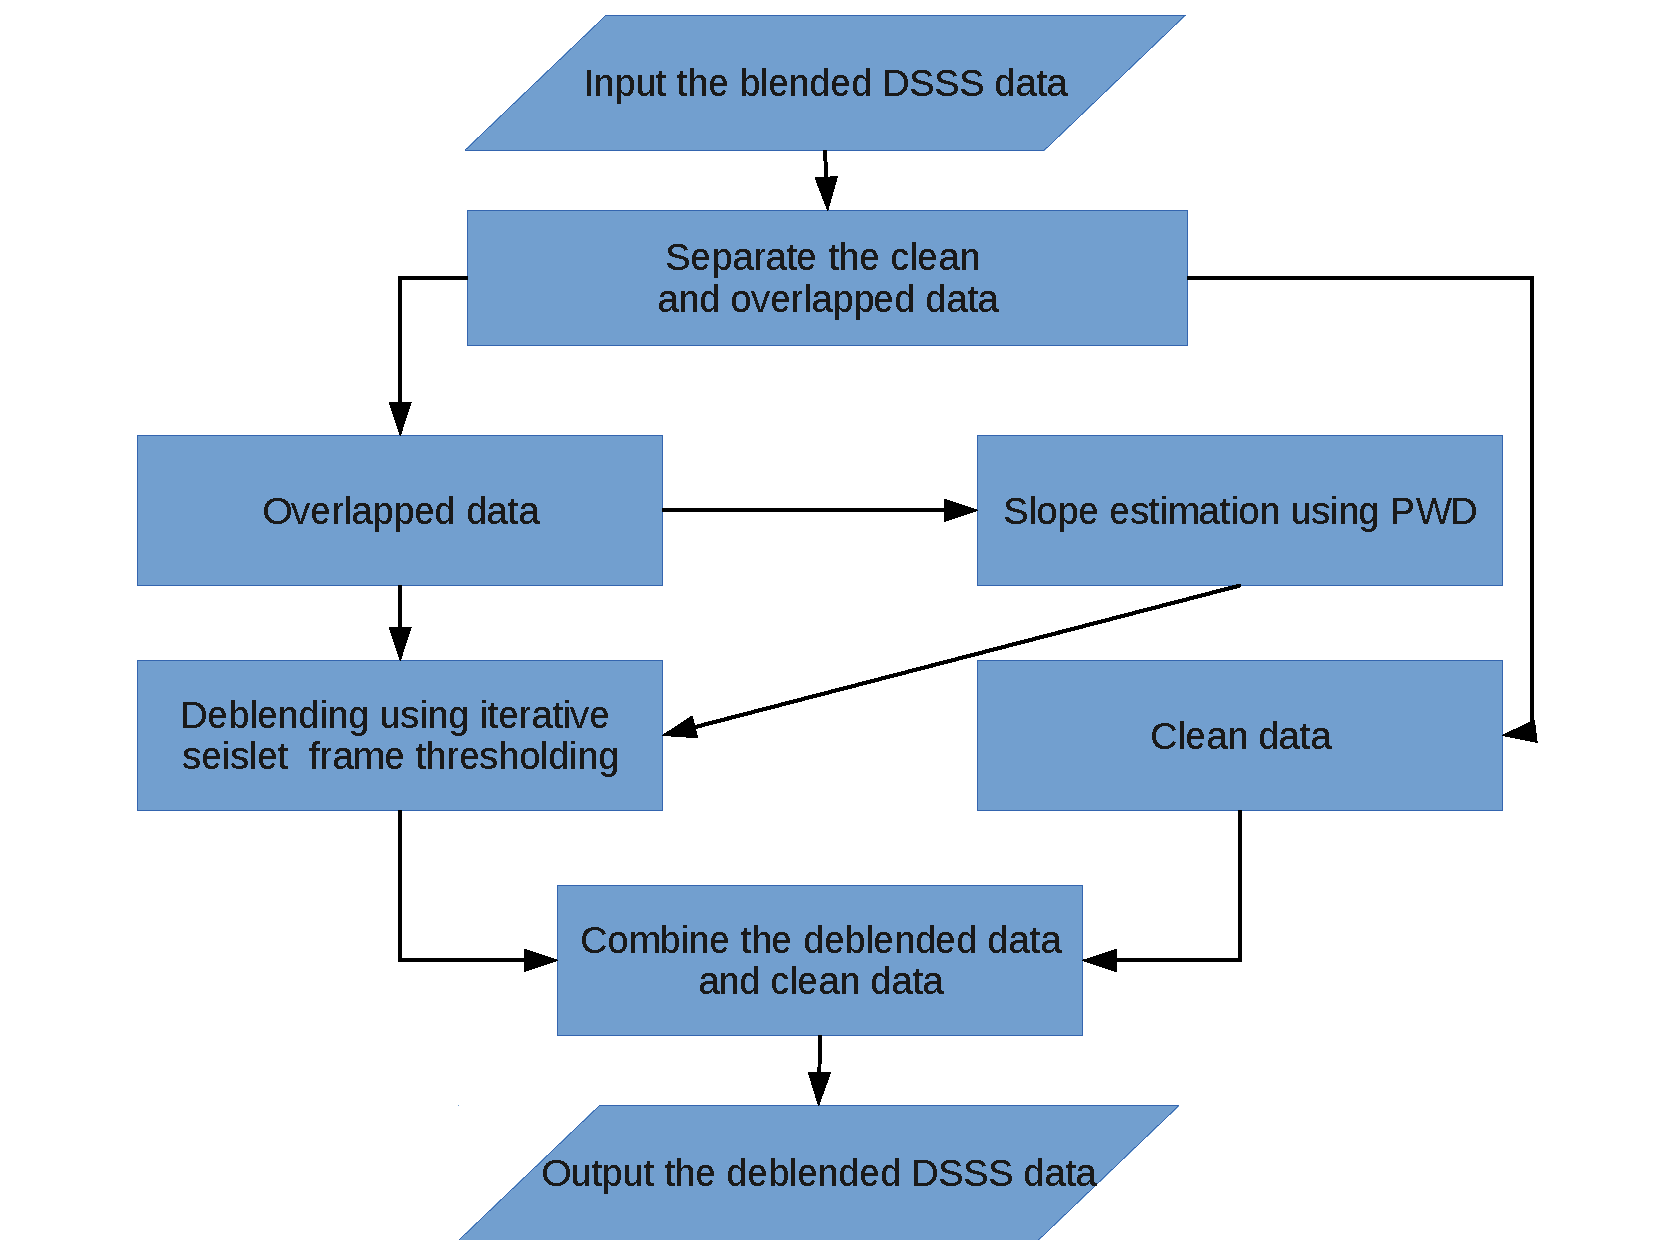
\includegraphics[width=0.6\columnwidth]{Fig/flowchart}          
   \caption{Flowchart of the algorithm.}
   \label{fig:flowchart}
\end{figure}


\begin{figure}[htb!]
  \centering
  \subfloat[]{\includegraphics[width=0.4\columnwidth]{syn1/Fig/syn1-c}
    \label{fig:syn1-c}}
  \subfloat[]{\includegraphics[width=0.4\columnwidth]{syn1/Fig/syn1}
    \label{fig:syn1}}            
   \caption{2D synthetic example. (a) Clean data. (b) Noisy data.}
   \label{fig:syn1}
\end{figure}

\begin{figure}[htb!]
  \centering
  \subfloat[]{\includegraphics[width=0.4\columnwidth]{syn1/Fig/syn1-ssa}
    \label{fig:syn1-ssa}}
  \subfloat[]{\includegraphics[width=0.4\columnwidth]{syn1/Fig/syn1-sst}
    \label{fig:syn1-sst}} \\
  \subfloat[]{\includegraphics[width=0.4\columnwidth]{syn1/Fig/syn1-ssa-n}
    \label{fig:syn1-ssa-n}}
  \subfloat[]{\includegraphics[width=0.4\columnwidth]{syn1/Fig/syn1-sst-n}
    \label{fig:syn1-sst-n}}             
   \caption{Denoising comparison. (a) Denoised data using SSA. (b) Denoised data using OSST. (c) Removed noise using SSA. (d) Removed noise using OSST.}
   \label{fig:syn1-dn}
\end{figure}

\begin{figure}[htb!]
  \centering
  \includegraphics[width=\columnwidth]{syn1/Fig/snr-n}        
   \caption{Output SNRs varying with different input noise level. The noise level is measured by noise variance.}
   \label{fig:snr-n}
\end{figure}

\begin{figure}[htb!]
  \centering
  \subfloat[]{\includegraphics[width=0.3\columnwidth]{syn1/Fig/syn1-sp}
    \label{fig:syn1-sp}}
  \subfloat[]{\includegraphics[width=0.3\columnwidth]{syn1/Fig/syn1-sp-ssa}
    \label{fig:syn1-sp-ssa}}
  \subfloat[]{\includegraphics[width=0.3\columnwidth]{syn1/Fig/syn1-sp-sst}
    \label{fig:syn1-sp-sst}} \\
  \subfloat[]{\includegraphics[width=0.3\columnwidth]{syn1/Fig/syn1-sp-ssa-n}
    \label{fig:syn1-sp-ssa-n}}
  \subfloat[]{\includegraphics[width=0.3\columnwidth]{syn1/Fig/syn1-sp-sst-n}
    \label{fig:syn1-sp-sst-n}}             
   \caption{Spiky noise test. (a) Denoised data using SSA. (b) Denoised data using OSST. (c) Removed noise using SSA. (d) Removed noise using OSST. SNRs of (a),(b),(c) are 2.24 dB, 16.73 dB, and 18.97 dB, respectively.}
   \label{fig:syn1-sp-dn}
\end{figure}

\begin{figure}[htb!]
  \centering
  \subfloat[]{\includegraphics[width=0.3\columnwidth]{syn1/Fig/syn1-bd}
    \label{fig:syn1-bd}}
  \subfloat[]{\includegraphics[width=0.3\columnwidth]{syn1/Fig/syn1-bd-ssa}
    \label{fig:syn1-bd-ssa}}
  \subfloat[]{\includegraphics[width=0.3\columnwidth]{syn1/Fig/syn1-bd-sst}
    \label{fig:syn1-bd-sst}} \\
  \subfloat[]{\includegraphics[width=0.3\columnwidth]{syn1/Fig/syn1-bd-ssa-n}
    \label{fig:syn1-bd-ssa-n}}
  \subfloat[]{\includegraphics[width=0.3\columnwidth]{syn1/Fig/syn1-bd-sst-n}
    \label{fig:syn1-bd-sst-n}}             
   \caption{Blending noise test. (a) Denoised data using SSA. (b) Denoised data using OSST. (c) Removed noise using SSA. (d) Removed noise using OSST. SNRs of (a),(b),(c) are 0.85 dB, 12.23 dB, 15.15 dB, respectively.}
   \label{fig:syn1-bd-dn}
\end{figure}

\begin{figure}[htb!]
  \centering
  \subfloat[]{\includegraphics[width=0.3\columnwidth]{syn1/Fig/syn1-noise}
    \label{fig:syn1-noise}}
  \subfloat[]{\includegraphics[width=0.3\columnwidth]{syn1/Fig/syn1-ssak1}
    \label{fig:syn1-ssak1}}
  \subfloat[]{\includegraphics[width=0.3\columnwidth]{syn1/Fig/syn1-sstk1}
    \label{fig:syn1-sstk1}} \\
  \subfloat[]{\includegraphics[width=0.3\columnwidth]{syn1/Fig/syn1-ssak3}
    \label{fig:syn1-ssak3}}
  \subfloat[]{\includegraphics[width=0.3\columnwidth]{syn1/Fig/syn1-sstk3}
    \label{fig:syn1-sstk3}}             
   \caption{Test of applying \dlo{SSA}\wen{TSVD-based SSA} and \dlo{OSST}\wen{GROUSE-based SSA} methods to pure random noise. (a) Pure random noise. (b) Result from \dlo{SSA}\wen{TSVD-based SSA} with $K=1$. (c) Result from \dlo{OSST}\wen{GROUSE-based SSA} with $K=1$. (d) Result from \dlo{SSA}\wen{TSVD-based SSA} with $K=3$. (e) Result from \dlo{OSST}\wen{GROUSE-based SSA} with $K=3$. Note that the \dlo{SSA}\wen{TSVD-based SSA} method approximates stronger noise than \dlo{OSST}\wen{GROUSE-based SSA} method for the same predefined rank $K$}
   \label{fig:syn1-nssat}
\end{figure}

\begin{figure}[htb!]
  \centering
  \includegraphics[width=\columnwidth]{syn1/Fig/e-n}        
   \caption{Noise approximation test. Note that the \dlo{SSA}\wen{TSVD-based SSA} method approximates stronger noise than \dlo{OSST}\wen{GROUSE-based SSA} method for the same predefined rank $K$. }
   \label{fig:e-n}
\end{figure}

\begin{figure}[htb!]
  \centering
  \includegraphics[width=\columnwidth]{Fig/demo_random}        
   \caption{\new{Demonstration for the influence of the randomization operator to the random property of unwanted-noise.}}
   \label{fig:test_random}
\end{figure}


\begin{figure}[htb!]
  \centering
  \subfloat[]{\includegraphics[width=0.3\columnwidth]{hyper/Fig/hyper-coh}
    \label{fig:hyper-coh}}
  \subfloat[]{\includegraphics[width=0.3\columnwidth]{hyper/Fig/hyper-s-dn}
    \label{fig:hyper-s-dn}}
  \subfloat[]{\includegraphics[width=0.3\columnwidth]{hyper/Fig/hyper-s-dn2}
    \label{fig:hyper-s-dn2}}    \\
      \subfloat[]{\includegraphics[width=0.3\columnwidth]{hyper/Fig/hyper-sn}
    \label{fig:hyper-sn}} 
  \subfloat[]{\includegraphics[width=0.3\columnwidth]{hyper/Fig/hyper-s-dnn}
    \label{fig:hyper-s-dnn}}           
  \subfloat[]{\includegraphics[width=0.3\columnwidth]{hyper/Fig/hyper-s-dnn2}
    \label{fig:hyper-s-dnn2}}     
   \caption{Coherent noise test. (a) Noisy data containing coherent noise. (b) Denoised data using the \dlo{SSA}\wen{TSVD-based SSA} method. (b) Denoised data using the proposed method. (d) Randomized data using the method proposed in \cite{weilin2017}.  (e) Removed noise including both random and coherent noise using the \dlo{SSA}\wen{TSVD-based SSA} method. (f) Removed noise including both random and coherent noise  using the proposed method.}
   \label{fig:coh}
\end{figure}

\begin{figure}[htb!]
  \centering
  \subfloat[]{\includegraphics[width=0.45\columnwidth]{liuwei1/Fig/syn-c}
    \label{fig:syn-c}}
  \subfloat[]{\includegraphics[width=0.45\columnwidth]{liuwei1/Fig/syn}
    \label{fig:syn}}            
   \caption{2D synthetic example. (a) Clean data. (b) Noisy data. SNR of (b) is 0.73 dB.}
   \label{fig:syn-c,syn}
\end{figure}


\begin{figure}[htb!]
  \centering
  \subfloat[]{\includegraphics[width=0.45\columnwidth]{liuwei1/Fig/syn-ssa}
    \label{fig:syn-ssa}}
  \subfloat[]{\includegraphics[width=0.45\columnwidth]{liuwei1/Fig/syn-sst}
    \label{fig:syn-sst}} \\
  \subfloat[]{\includegraphics[width=0.45\columnwidth]{liuwei1/Fig/syn-ssa-dif}
    \label{fig:syn-ssa-dif}}
  \subfloat[]{\includegraphics[width=0.45\columnwidth]{liuwei1/Fig/syn-sst-dif}
    \label{fig:syn-sst-dif}}             
   \caption{Denoising comparison. (a) Denoised data using SSA. (b) Denoised data using OSST. (c) Removed noise corresponding to (a). (d) Removed noise corresponding to (b). SNRs of (a) and (b) are 5.10 dB and 7.22 dB, respectively.}
   \label{fig:syn-dn}
\end{figure}


\begin{figure}[htb!]
  \centering
  \subfloat[]{\includegraphics[width=0.45\columnwidth]{liuwei1/Fig/syn-c-fk}
    \label{fig:syn-c-fk}}
  \subfloat[]{\includegraphics[width=0.45\columnwidth]{liuwei1/Fig/syn-fk}
    \label{fig:syn-fk}} \\
  \subfloat[]{\includegraphics[width=0.45\columnwidth]{liuwei1/Fig/syn-ssa-fk}
    \label{fig:syn-ssa-fk}}
  \subfloat[]{\includegraphics[width=0.45\columnwidth]{liuwei1/Fig/syn-sst-fk}
    \label{fig:syn-sst-fk}}             
   \caption{FK spectrum comparison. (a) FK spectrum of clean data. (b) FK spectrum of noisy data. (c) FK spectrum of \dlo{SSA}\wen{TSVD-based SSA} processed data. (d) FK spectrum of \dlo{OSST}\wen{GROUSE-based SSA} processed data.}
   \label{fig:syn-dnfk}
\end{figure}




\begin{figure}[htb!]
  \centering
  \subfloat[]{\includegraphics[width=0.4\columnwidth]{syn3d/Fig/syn3d-c}
    \label{fig:syn3d-c}}
  \subfloat[]{\includegraphics[width=0.4\columnwidth]{syn3d/Fig/syn3d-n}
    \label{fig:syn3d-n}}           
   \caption{3D synthetic example. (a) Clean data. (b) Noisy data.}
   \label{fig:syn3d-c,syn3d-n}
\end{figure}

\begin{figure}[htb!]
  \centering
  \subfloat[]{\includegraphics[width=0.4\columnwidth]{syn3d/Fig/syn3d-fk}
    \label{fig:syn3d-fk}}
  \subfloat[]{\includegraphics[width=0.4\columnwidth]{syn3d/Fig/syn3d-ssa}
    \label{fig:syn3d-mssa}}  \\ 
  \subfloat[]{\includegraphics[width=0.4\columnwidth]{syn3d/Fig/syn3d-rsvd}
    \label{fig:syn3d-rsvd}}
  \subfloat[]{\includegraphics[width=0.4\columnwidth]{syn3d/Fig/syn3d-mc}
    \label{fig:syn3d-mc}}        
   \caption{Denoising comparison.  (a) Denoised data using FK method. (b) Denoised data using \dlo{SSA}\wen{TSVD-based SSA} method with SVD for low-rank decomposition. (c) Denoised data using \dlo{SSA}\wen{TSVD-based SSA} method with RSVD for low-rank decomposition. (d) Denoised data using \dlo{OSST}\wen{GROUSE-based SSA} method via GROUSE for low-rank decomposition.}
   \label{fig:syn3d-fk,syn3d-mssa,syn3d-rsvd,syn3d-mc}
\end{figure}

\begin{figure}[htb!]
  \centering
  \subfloat[]{\includegraphics[width=0.4\columnwidth]{syn3d/Fig/syn3d-n-fk}
    \label{fig:syn3d-n-fk}}
  \subfloat[]{\includegraphics[width=0.4\columnwidth]{syn3d/Fig/syn3d-n-ssa}
    \label{fig:syn3d-n-mssa}}  \\ 
  \subfloat[]{\includegraphics[width=0.4\columnwidth]{syn3d/Fig/syn3d-n-rsvd}
    \label{fig:syn3d-n-rsvd}}
  \subfloat[]{\includegraphics[width=0.4\columnwidth]{syn3d/Fig/syn3d-n-mc}
    \label{fig:syn3d-n-mc}}        
   \caption{Noise comparison. (a) Removed noise using FK method. (b) Removed noise using \dlo{SSA}\wen{TSVD-based SSA} method with SVD for low-rank decomposition. (c) Removed noise using \dlo{SSA}\wen{TSVD-based SSA} method with RSVD for low-rank decomposition. (d) Removed noise using \dlo{OSST}\wen{GROUSE-based SSA} method via GROUSE for low-rank decomposition.}
   \label{fig:syn3d-n-fk,syn3d-n-mssa,syn3d-n-rsvd,syn3d-n-mc}
\end{figure}

\begin{figure}[htb!]
  \centering
  \subfloat[]{\includegraphics[width=0.3\columnwidth]{syn3d/Fig/syn3d-c-s}
    \label{fig:syn3d-c-s}}
  \subfloat[]{\includegraphics[width=0.3\columnwidth]{syn3d/Fig/syn3d-fk-s}
    \label{fig:syn3d-fk-s}}
  \subfloat[]{\includegraphics[width=0.3\columnwidth]{syn3d/Fig/syn3d-ssa-s}
    \label{fig:syn3d-ssa-s}}  \\ 
  \subfloat[]{\includegraphics[width=0.3\columnwidth]{syn3d/Fig/syn3d-n-s}
    \label{fig:syn3d-n-s}}
  \subfloat[]{\includegraphics[width=0.3\columnwidth]{syn3d/Fig/syn3d-rsvd-s}
    \label{fig:syn3d-rsvd-s}}
  \subfloat[]{\includegraphics[width=0.3\columnwidth]{syn3d/Fig/syn3d-mc-s}
    \label{fig:syn3d-mc-s}}        
   \caption{2D section comparison (5th Xline section). (a) Clean data. (b) Denoised data using FK. (c) Denoised data using SSA. (d) Noisy data. (e) Denoised data using RSVD. (f) Denoised data using OSST.}
   \label{fig:syn3d-c-s,syn3d-fk-s,syn3d-ssa-s,syn3d-n-s,syn3d-rsvd-s,syn3d-mc-s}
\end{figure}

\begin{figure}[htb!]
  \centering
  \includegraphics[width=0.7\columnwidth]{guochang/Fig/real}          
   \caption{2D field data example.}
   \label{fig:real}
\end{figure}

\begin{figure}[htb!]
  \centering
  \subfloat[]{\includegraphics[width=0.7\columnwidth]{guochang/Fig/r-ssa}
    \label{fig:r-ssa}}\\
  \subfloat[]{\includegraphics[width=0.7\columnwidth]{guochang/Fig/r-sst}
    \label{fig:r-sst}}            
   \caption{Denoising comparison. (a) Denoised data using SSA. (b) Denoised data using OSST. }
   \label{fig:real-dn}
\end{figure}

\begin{figure}[htb!]
  \centering
  \subfloat[]{\includegraphics[width=0.7\columnwidth]{guochang/Fig/r-ssa-n-0}
    \label{fig:r-ssa-n}}\\
  \subfloat[]{\includegraphics[width=0.7\columnwidth]{guochang/Fig/r-sst-n-0}
    \label{fig:r-sst-n}}            
   \caption{Denoising comparison. (a) Removed noise using SSA. (d) Removed noise using OSST. \wen{The zoomed sections of the frameboxes are shown in Figure \ref{fig:real-n-z}.}}
   \label{fig:real-n}
\end{figure}

\begin{figure}[htb!]
  \centering
  \subfloat[]{\includegraphics[width=0.7\columnwidth]{guochang/Fig/r-ssa-n-z}
    \label{fig:r-ssa-n-z}}\\
  \subfloat[]{\includegraphics[width=0.7\columnwidth]{guochang/Fig/r-sst-n-z}
    \label{fig:r-sst-n-z}}            
   \caption{\wen{Zoomed denoising comparison}\dlo{Denoising comparison}. (a) Removed noise using SSA. (d) Removed noise using OSST.}
   \label{fig:real-n-z}
\end{figure}

\begin{figure}[htb!]
  \centering
  \subfloat[]{\includegraphics[width=0.7\columnwidth]{guochang/Fig/r-ssa-simi-0}
    \label{fig:r-ssa-simi}}\\
  \subfloat[]{\includegraphics[width=0.7\columnwidth]{guochang/Fig/r-sst-simi-0}
    \label{fig:r-sst-simi}}            
   \caption{Denoising comparison in terms of local similarity between denoised data and removed noise. (a) Local similarity using SSA. (d) Local similarity using OSST.}
   \label{fig:real-simi}
\end{figure}

\begin{figure}[htb!]
  \centering
  \includegraphics[width=0.7\columnwidth]{field/Fig/field}          
   \caption{3D field data example.}
   \label{fig:field}
\end{figure}

\begin{figure}[htb!]
  \centering
  \subfloat[]{\includegraphics[width=0.4\columnwidth]{field/Fig/field-ssa}
    \label{fig:field-ssa}}
  \subfloat[]{\includegraphics[width=0.4\columnwidth]{field/Fig/field-sst}
    \label{fig:field-sst}} \\
  \subfloat[]{\includegraphics[width=0.4\columnwidth]{field/Fig/field-n-ssa}
    \label{fig:field-n-ssa}}
  \subfloat[]{\includegraphics[width=0.4\columnwidth]{field/Fig/field-n-sst}
    \label{fig:field-n-sst}}            
   \caption{Denoising comparison in 3D volume. (a) Denoised data using SSA. (b) Denoised data using OSST. (c) Removed noise corresponding (a). (d) Removed noise corresponding to (b).}
   \label{fig:field-3d}
\end{figure}

\begin{figure}[htb!]
  \centering
  \subfloat[]{\includegraphics[width=0.48\columnwidth]{field/Fig/f-ssa-simi}
    \label{fig:f-ssa-simi}}
  \subfloat[]{\includegraphics[width=0.48\columnwidth]{field/Fig/f-sst-simi}
    \label{fig:f-sst-simi}}          
   \caption{Denoising comparison in terms of local similarity between denoised data and removed noise. (a) Local similarity using \dlo{SSA}\wen{TSVD-based SSA} method. (b) Local similarity using \dlo{OSST}\wen{GROUSE-based SSA} method.}
   \label{fig:fsimi}
\end{figure}


\begin{figure}[htb!]
  \centering
  \subfloat[]{\includegraphics[width=0.32\columnwidth]{field/Fig/field-s-0}
    \label{fig:field-s}}
  \subfloat[]{\includegraphics[width=0.32\columnwidth]{field/Fig/field-s-ssa-0}
    \label{fig:field-s-ssa}}
  \subfloat[]{\includegraphics[width=0.32\columnwidth]{field/Fig/field-s-sst-0}
    \label{fig:field-s-sst}} \\
  \subfloat[]{\includegraphics[width=0.32\columnwidth]{field/Fig/field-sn-ssa}
    \label{fig:field-sn-ssa}}
  \subfloat[]{\includegraphics[width=0.32\columnwidth]{field/Fig/field-sn-sst}
    \label{fig:field-sn-sst}}            
   \caption{Denoising comparison in 2D section. (a) Raw seismic data. (b) Denoised data using SSA. (c) Denoised data using OSST. (d) Removed noise corresponding (a). (e) Removed noise corresponding to (b).}
   \label{fig:field-2d}
\end{figure}

\begin{figure}[htb!]
  \centering
  \subfloat[]{\includegraphics[width=0.45\columnwidth]{field/Fig/z-field}
    \label{fig:z-field}}\\
  \subfloat[]{\includegraphics[width=0.45\columnwidth]{field/Fig/z-ssa}
    \label{fig:z-ssa}}
  \subfloat[]{\includegraphics[width=0.45\columnwidth]{field/Fig/z-sst}
    \label{fig:z-sst}}          
   \caption{Zoomed comparison. (a) Raw seismic data. (b) Denoised data using SSA. (c) Denoised data using OSST.}
   \label{fig:field-z}
\end{figure}


%\begin{figure}[htb!]
%  \centering
%  \subfloat[]{\includegraphics[width=0.48\columnwidth]{earthquake/Fig/reftran}
%    \label{fig:reftran}}\\
%  \subfloat[]{\includegraphics[width=0.48\columnwidth]{earthquake/Fig/ref-sst}
%    \label{fig:ref-sst}}
%  \subfloat[]{\includegraphics[width=0.48\columnwidth]{earthquake/Fig/ref-sst-n}
%    \label{fig:ref-sst-n}}          
%   \caption{(a) Raw stack data. (b) Denoised stack. (c) Removed noise.}
%   \label{fig:earth}
%\end{figure}

\begin{figure}[htb!]
  \centering
  \includegraphics[width=0.95\columnwidth]{earthquake/Fig/reftran}     
   \caption{Raw earthquake stack data. }
   \label{fig:reftran}
\end{figure}

\begin{figure}[htb!]
  \centering
  \includegraphics[width=0.95\columnwidth]{earthquake/Fig/ref-sst}
       
   \caption{Denoised stack data. }
    \label{fig:ref-sst} 
\end{figure}

\begin{figure}[htb!]
  \centering
  \includegraphics[width=0.95\columnwidth]{earthquake/Fig/ref-sst-n}
       
   \caption{Removed noise from the raw earthquake stack data.}
    \label{fig:ref-sst-n}  
\end{figure}


